\documentclass[twoside]{book}

% Packages required by doxygen
\usepackage{fixltx2e}
\usepackage{calc}
\usepackage{doxygen}
\usepackage[export]{adjustbox} % also loads graphicx
\usepackage{graphicx}
\usepackage[utf8]{inputenc}
\usepackage{makeidx}
\usepackage{multicol}
\usepackage{multirow}
\PassOptionsToPackage{warn}{textcomp}
\usepackage{textcomp}
\usepackage[nointegrals]{wasysym}
\usepackage[table]{xcolor}

% NLS support packages
\usepackage[french]{babel}

% Font selection
\usepackage[T1]{fontenc}
\usepackage[scaled=.90]{helvet}
\usepackage{courier}
\usepackage{amssymb}
\usepackage{sectsty}
\renewcommand{\familydefault}{\sfdefault}
\allsectionsfont{%
  \fontseries{bc}\selectfont%
  \color{darkgray}%
}
\renewcommand{\DoxyLabelFont}{%
  \fontseries{bc}\selectfont%
  \color{darkgray}%
}
\newcommand{\+}{\discretionary{\mbox{\scriptsize$\hookleftarrow$}}{}{}}

% Page & text layout
\usepackage{geometry}
\geometry{%
  a4paper,%
  top=2.5cm,%
  bottom=2.5cm,%
  left=2.5cm,%
  right=2.5cm%
}
\tolerance=750
\hfuzz=15pt
\hbadness=750
\setlength{\emergencystretch}{15pt}
\setlength{\parindent}{0cm}
\setlength{\parskip}{3ex plus 2ex minus 2ex}
\makeatletter
\renewcommand{\paragraph}{%
  \@startsection{paragraph}{4}{0ex}{-1.0ex}{1.0ex}{%
    \normalfont\normalsize\bfseries\SS@parafont%
  }%
}
\renewcommand{\subparagraph}{%
  \@startsection{subparagraph}{5}{0ex}{-1.0ex}{1.0ex}{%
    \normalfont\normalsize\bfseries\SS@subparafont%
  }%
}
\makeatother

% Headers & footers
\usepackage{fancyhdr}
\pagestyle{fancyplain}
\fancyhead[LE]{\fancyplain{}{\bfseries\thepage}}
\fancyhead[CE]{\fancyplain{}{}}
\fancyhead[RE]{\fancyplain{}{\bfseries\leftmark}}
\fancyhead[LO]{\fancyplain{}{\bfseries\rightmark}}
\fancyhead[CO]{\fancyplain{}{}}
\fancyhead[RO]{\fancyplain{}{\bfseries\thepage}}
\fancyfoot[LE]{\fancyplain{}{}}
\fancyfoot[CE]{\fancyplain{}{}}
\fancyfoot[RE]{\fancyplain{}{\bfseries\scriptsize Généré par Doxygen }}
\fancyfoot[LO]{\fancyplain{}{\bfseries\scriptsize Généré par Doxygen }}
\fancyfoot[CO]{\fancyplain{}{}}
\fancyfoot[RO]{\fancyplain{}{}}
\renewcommand{\footrulewidth}{0.4pt}
\renewcommand{\chaptermark}[1]{%
  \markboth{#1}{}%
}
\renewcommand{\sectionmark}[1]{%
  \markright{\thesection\ #1}%
}

% Indices & bibliography
\usepackage{natbib}
\usepackage[titles]{tocloft}
\setcounter{tocdepth}{3}
\setcounter{secnumdepth}{5}
\makeindex

% Hyperlinks (required, but should be loaded last)
\usepackage{ifpdf}
\ifpdf
  \usepackage[pdftex,pagebackref=true]{hyperref}
\else
  \usepackage[ps2pdf,pagebackref=true]{hyperref}
\fi
\hypersetup{%
  colorlinks=true,%
  linkcolor=blue,%
  citecolor=blue,%
  unicode%
}

% Custom commands
\newcommand{\clearemptydoublepage}{%
  \newpage{\pagestyle{empty}\cleardoublepage}%
}

\usepackage{caption}
\captionsetup{labelsep=space,justification=centering,font={bf},singlelinecheck=off,skip=4pt,position=top}

%===== C O N T E N T S =====

\begin{document}

% Titlepage & ToC
\hypersetup{pageanchor=false,
             bookmarksnumbered=true,
             pdfencoding=unicode
            }
\pagenumbering{roman}
\begin{titlepage}
\vspace*{7cm}
\begin{center}%
{\Large Tag\+Manager \\[1ex]\large 1.\+0 }\\
\vspace*{1cm}
{\large Généré par Doxygen 1.8.11}\\
\end{center}
\end{titlepage}
\clearemptydoublepage
\tableofcontents
\clearemptydoublepage
\pagenumbering{arabic}
\hypersetup{pageanchor=true}

%--- Begin generated contents ---
\chapter{Tag\+Manager}
\label{md_README}
\hypertarget{md_README}{}
Dans le module I\+HM encadré par Eric Languenou de notre formation (Master 1 A\+L\+MA U\+FR Nantes 2016/2016), nous devions créer une application qui permet de créer des tags et donc d\textquotesingle{}associer différents fichiers/dossiers à ces tags et d\textquotesingle{}effectuer une recherche en OU logique et ET logique.

\section*{Programmeurs}


\begin{DoxyItemize}
\item Killian Gomes
\item Sullivan Pineau
\end{DoxyItemize}

\section*{Lancer cette application}

Effectuer les différentes commandes dans le repertoire courant de l\textquotesingle{}application via un terminal \+:

\begin{quote}
qmake \end{quote}


\begin{quote}
make \end{quote}


\begin{quote}
./\+Tag\+Manager\end{quote}

\chapter{Index hiérarchique}
\section{Hiérarchie des classes}
Cette liste d\textquotesingle{}héritage est classée approximativement par ordre alphabétique \+:\begin{DoxyCompactList}
\item Q\+Push\+Button\begin{DoxyCompactList}
\item \contentsline{section}{Q\+Push\+Button\+Plus}{\pageref{class_q_push_button_plus}}{}
\end{DoxyCompactList}
\item Q\+Table\+View\begin{DoxyCompactList}
\item \contentsline{section}{My\+View}{\pageref{class_my_view}}{}
\end{DoxyCompactList}
\item Q\+Widget\begin{DoxyCompactList}
\item \contentsline{section}{Q\+WidgetO}{\pageref{class_q_widget_o}}{}
\begin{DoxyCompactList}
\item \contentsline{section}{Tab\+Edition}{\pageref{class_tab_edition}}{}
\item \contentsline{section}{Tab\+Recherche}{\pageref{class_tab_recherche}}{}
\end{DoxyCompactList}
\end{DoxyCompactList}
\item \contentsline{section}{Style}{\pageref{class_style}}{}
\item \contentsline{section}{Tag}{\pageref{class_tag}}{}
\item \contentsline{section}{Tags}{\pageref{class_tags}}{}
\end{DoxyCompactList}

\chapter{Index des classes}
\section{Liste des classes}
Liste des classes, structures, unions et interfaces avec une brève description \+:\begin{DoxyCompactList}
\item\contentsline{section}{\hyperlink{class_my_view}{My\+View} \\*Classe permettant de redéfinir la classe Q\+Table\+View }{\pageref{class_my_view}}{}
\item\contentsline{section}{\hyperlink{class_q_push_button_plus}{Q\+Push\+Button\+Plus} \\*Classe permettant de redéfinir la classe Q\+Push\+Button }{\pageref{class_q_push_button_plus}}{}
\item\contentsline{section}{\hyperlink{class_q_widget_o}{Q\+WidgetO} \\*Classe permettant de redéfinir la classe Q\+Widget }{\pageref{class_q_widget_o}}{}
\item\contentsline{section}{\hyperlink{class_style}{Style} \\*Classe permettant de définir la classe \hyperlink{class_style}{Style} }{\pageref{class_style}}{}
\item\contentsline{section}{\hyperlink{class_tab_edition}{Tab\+Edition} \\*Classe permettant de définir la classe \hyperlink{class_tab_edition}{Tab\+Edition} }{\pageref{class_tab_edition}}{}
\item\contentsline{section}{\hyperlink{class_tab_recherche}{Tab\+Recherche} \\*Classe permettant de définir la classe \hyperlink{class_tab_recherche}{Tab\+Recherche} }{\pageref{class_tab_recherche}}{}
\item\contentsline{section}{\hyperlink{class_tag}{Tag} \\*Classe permettant de représenter un tag (chaque tag possède un nom et une liste de chemin qui lui ont été associé) }{\pageref{class_tag}}{}
\item\contentsline{section}{\hyperlink{class_tags}{Tags} \\*Classe permettant de lister les différents tags et possède un pointeur vers les deux modes }{\pageref{class_tags}}{}
\end{DoxyCompactList}

\chapter{Index des fichiers}
\section{Liste des fichiers}
Liste de tous les fichiers documentés avec une brève description \+:\begin{DoxyCompactList}
\item\contentsline{section}{Headers/\hyperlink{_my_view_8h}{My\+View.\+h} \\*Définition d\textquotesingle{}une classe de \hyperlink{class_my_view}{My\+View} }{\pageref{_my_view_8h}}{}
\item\contentsline{section}{Headers/{\bfseries Q\+Push\+Button\+Plus.\+h} }{\pageref{_q_push_button_plus_8h}}{}
\item\contentsline{section}{Headers/\hyperlink{_q_widget_o_8h}{Q\+Widget\+O.\+h} \\*Définition d\textquotesingle{}une classe de \hyperlink{class_q_widget_o}{Q\+WidgetO} }{\pageref{_q_widget_o_8h}}{}
\item\contentsline{section}{Headers/\hyperlink{_style_8h}{Style.\+h} \\*Définition d\textquotesingle{}une classe de \hyperlink{class_style}{Style} }{\pageref{_style_8h}}{}
\item\contentsline{section}{Headers/\hyperlink{_tab_edition_8h}{Tab\+Edition.\+h} \\*Définition d\textquotesingle{}une classe de \hyperlink{class_tab_edition}{Tab\+Edition} }{\pageref{_tab_edition_8h}}{}
\item\contentsline{section}{Headers/\hyperlink{_tab_recherche_8h}{Tab\+Recherche.\+h} \\*Définition d\textquotesingle{}une classe de \hyperlink{class_tab_recherche}{Tab\+Recherche} }{\pageref{_tab_recherche_8h}}{}
\item\contentsline{section}{Headers/\hyperlink{_tag_8h}{Tag.\+h} \\*Définition d\textquotesingle{}une classe de Tab }{\pageref{_tag_8h}}{}
\item\contentsline{section}{Headers/\hyperlink{_tags_8h}{Tags.\+h} \\*Définition d\textquotesingle{}une classe de Tabs }{\pageref{_tags_8h}}{}
\item\contentsline{section}{Sources/\hyperlink{_q_push_button_plus_8cpp}{Q\+Push\+Button\+Plus.\+cpp} \\*Implémentation des méthodes de la classe \hyperlink{class_q_push_button_plus}{Q\+Push\+Button\+Plus} }{\pageref{_q_push_button_plus_8cpp}}{}
\item\contentsline{section}{Sources/\hyperlink{_style_8cpp}{Style.\+cpp} \\*Implémentation de la méthode de la classe \hyperlink{class_style}{Style} }{\pageref{_style_8cpp}}{}
\item\contentsline{section}{Sources/\hyperlink{_tab_edition_8cpp}{Tab\+Edition.\+cpp} \\*Implémentation des méthodes de la classe \hyperlink{class_tab_edition}{Tab\+Edition} }{\pageref{_tab_edition_8cpp}}{}
\item\contentsline{section}{Sources/\hyperlink{_tab_recherche_8cpp}{Tab\+Recherche.\+cpp} \\*Implémentation des méthodes de la classe \hyperlink{class_q_push_button_plus}{Q\+Push\+Button\+Plus} }{\pageref{_tab_recherche_8cpp}}{}
\item\contentsline{section}{Sources/\hyperlink{_tags_8cpp}{Tags.\+cpp} \\*Implémentation des méthodes de la classe Tabs }{\pageref{_tags_8cpp}}{}
\end{DoxyCompactList}

\chapter{Documentation des classes}
\hypertarget{class_my_view}{}\section{Référence de la classe My\+View}
\label{class_my_view}\index{My\+View@{My\+View}}


Classe permettant de redéfinir la classe Q\+Table\+View.  




{\ttfamily \#include $<$My\+View.\+h$>$}



Graphe d\textquotesingle{}héritage de My\+View\+:\nopagebreak
\begin{figure}[H]
\begin{center}
\leavevmode
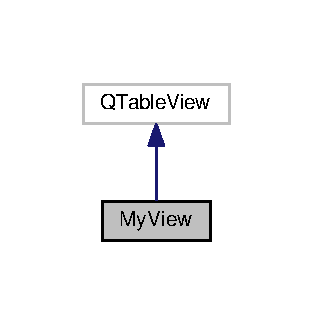
\includegraphics[width=150pt]{class_my_view__inherit__graph}
\end{center}
\end{figure}


Graphe de collaboration de My\+View\+:\nopagebreak
\begin{figure}[H]
\begin{center}
\leavevmode
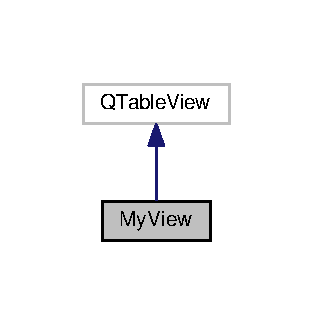
\includegraphics[width=150pt]{class_my_view__coll__graph}
\end{center}
\end{figure}
\subsection*{Signaux}
\begin{DoxyCompactItemize}
\item 
void \hyperlink{class_my_view_a94a8e0854d7c5b07f71c9ab71bf2bb56}{right\+Clicked} ()\hypertarget{class_my_view_a94a8e0854d7c5b07f71c9ab71bf2bb56}{}\label{class_my_view_a94a8e0854d7c5b07f71c9ab71bf2bb56}

\begin{DoxyCompactList}\small\item\em procédure permettant de réprésenter le signal d\textquotesingle{}un clic droit \end{DoxyCompactList}\item 
void \hyperlink{class_my_view_a845fd0cc0f988e65060d3eb367584583}{double\+Clicked} ()\hypertarget{class_my_view_a845fd0cc0f988e65060d3eb367584583}{}\label{class_my_view_a845fd0cc0f988e65060d3eb367584583}

\begin{DoxyCompactList}\small\item\em procédure permettant de réprésenter le signal d\textquotesingle{}un double clic \end{DoxyCompactList}\end{DoxyCompactItemize}
\subsection*{Fonctions membres publiques}
\begin{DoxyCompactItemize}
\item 
\hyperlink{class_my_view_ad3d369abeec4aedbe6701cb4452eb8c4}{My\+View} (Q\+Widget $\ast$parent=0)
\begin{DoxyCompactList}\small\item\em Constructeur, crée un objet Myview. \end{DoxyCompactList}\item 
Q\+Point \hyperlink{class_my_view_a55c1b10748589b3c32d2c03a175edbe5}{get\+Pos} ()
\begin{DoxyCompactList}\small\item\em Getter de l\textquotesingle{}attribut pos. \end{DoxyCompactList}\end{DoxyCompactItemize}


\subsection{Description détaillée}
Classe permettant de redéfinir la classe Q\+Table\+View. 

\subsection{Documentation des constructeurs et destructeur}
\index{My\+View@{My\+View}!My\+View@{My\+View}}
\index{My\+View@{My\+View}!My\+View@{My\+View}}
\subsubsection[{\texorpdfstring{My\+View(\+Q\+Widget $\ast$parent=0)}{MyView(QWidget *parent=0)}}]{\setlength{\rightskip}{0pt plus 5cm}My\+View\+::\+My\+View (
\begin{DoxyParamCaption}
\item[{Q\+Widget $\ast$}]{parent = {\ttfamily 0}}
\end{DoxyParamCaption}
)\hspace{0.3cm}{\ttfamily [explicit]}}\hypertarget{class_my_view_ad3d369abeec4aedbe6701cb4452eb8c4}{}\label{class_my_view_ad3d369abeec4aedbe6701cb4452eb8c4}


Constructeur, crée un objet Myview. 


\begin{DoxyParams}{Paramètres}
{\em Q\+Widget$\ast$,parent} & = 0 \\
\hline
\end{DoxyParams}


\subsection{Documentation des fonctions membres}
\index{My\+View@{My\+View}!get\+Pos@{get\+Pos}}
\index{get\+Pos@{get\+Pos}!My\+View@{My\+View}}
\subsubsection[{\texorpdfstring{get\+Pos()}{getPos()}}]{\setlength{\rightskip}{0pt plus 5cm}Q\+Point My\+View\+::get\+Pos (
\begin{DoxyParamCaption}
{}
\end{DoxyParamCaption}
)}\hypertarget{class_my_view_a55c1b10748589b3c32d2c03a175edbe5}{}\label{class_my_view_a55c1b10748589b3c32d2c03a175edbe5}


Getter de l\textquotesingle{}attribut pos. 

\begin{DoxyReturn}{Renvoie}
attribut pos 
\end{DoxyReturn}


La documentation de cette classe a été générée à partir des fichiers suivants \+:\begin{DoxyCompactItemize}
\item 
Headers/\hyperlink{_my_view_8h}{My\+View.\+h}\item 
Sources/My\+View.\+cpp\end{DoxyCompactItemize}

\hypertarget{class_q_push_button_plus}{}\section{Référence de la classe Q\+Push\+Button\+Plus}
\label{class_q_push_button_plus}\index{Q\+Push\+Button\+Plus@{Q\+Push\+Button\+Plus}}


Classe permettant de redéfinir la classe Q\+Push\+Button.  




{\ttfamily \#include $<$Q\+Push\+Button\+Plus.\+h$>$}



Graphe d\textquotesingle{}héritage de Q\+Push\+Button\+Plus\+:\nopagebreak
\begin{figure}[H]
\begin{center}
\leavevmode
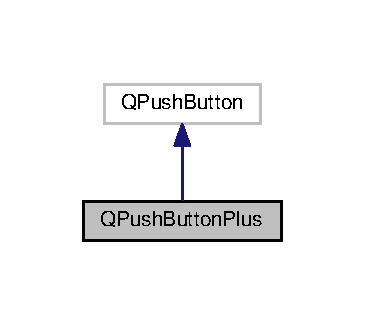
\includegraphics[width=175pt]{class_q_push_button_plus__inherit__graph}
\end{center}
\end{figure}


Graphe de collaboration de Q\+Push\+Button\+Plus\+:\nopagebreak
\begin{figure}[H]
\begin{center}
\leavevmode
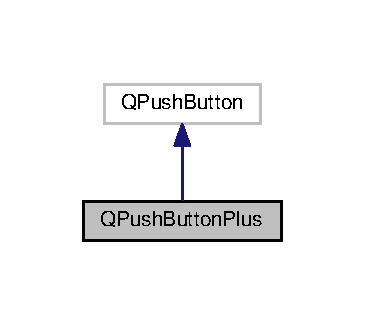
\includegraphics[width=175pt]{class_q_push_button_plus__coll__graph}
\end{center}
\end{figure}
\subsection*{Signaux}
\begin{DoxyCompactItemize}
\item 
void \hyperlink{class_q_push_button_plus_a8c120f8c9b33c2cd0d6282bc570559f3}{right\+Clicked} ()\hypertarget{class_q_push_button_plus_a8c120f8c9b33c2cd0d6282bc570559f3}{}\label{class_q_push_button_plus_a8c120f8c9b33c2cd0d6282bc570559f3}

\begin{DoxyCompactList}\small\item\em procédure permettant de réprésenter le signal d\textquotesingle{}un clic droit \end{DoxyCompactList}\item 
void \hyperlink{class_q_push_button_plus_a97c13206b568d3e4e83d7191703b9bab}{left\+Clicked} ()\hypertarget{class_q_push_button_plus_a97c13206b568d3e4e83d7191703b9bab}{}\label{class_q_push_button_plus_a97c13206b568d3e4e83d7191703b9bab}

\begin{DoxyCompactList}\small\item\em procédure permettant de réprésenter le signal d\textquotesingle{}un clic gauche \end{DoxyCompactList}\end{DoxyCompactItemize}
\subsection*{Fonctions membres publiques}
\begin{DoxyCompactItemize}
\item 
\hyperlink{class_q_push_button_plus_a0e4bf0e820b7401bb99cc7eb1d5b96b9}{Q\+Push\+Button\+Plus} (Q\+String name, Q\+Widget $\ast$parent=0)
\begin{DoxyCompactList}\small\item\em Constructeur, crée un objet \hyperlink{class_q_push_button_plus}{Q\+Push\+Button\+Plus}. \end{DoxyCompactList}\item 
Q\+Point \hyperlink{class_q_push_button_plus_a902660536c4021ac2bbbc2f5cca34301}{get\+Pos} ()
\begin{DoxyCompactList}\small\item\em Getter de l\textquotesingle{}attribut pos. \end{DoxyCompactList}\end{DoxyCompactItemize}


\subsection{Description détaillée}
Classe permettant de redéfinir la classe Q\+Push\+Button. 

\subsection{Documentation des constructeurs et destructeur}
\index{Q\+Push\+Button\+Plus@{Q\+Push\+Button\+Plus}!Q\+Push\+Button\+Plus@{Q\+Push\+Button\+Plus}}
\index{Q\+Push\+Button\+Plus@{Q\+Push\+Button\+Plus}!Q\+Push\+Button\+Plus@{Q\+Push\+Button\+Plus}}
\subsubsection[{\texorpdfstring{Q\+Push\+Button\+Plus(\+Q\+String name, Q\+Widget $\ast$parent=0)}{QPushButtonPlus(QString name, QWidget *parent=0)}}]{\setlength{\rightskip}{0pt plus 5cm}Q\+Push\+Button\+Plus\+::\+Q\+Push\+Button\+Plus (
\begin{DoxyParamCaption}
\item[{Q\+String}]{name, }
\item[{Q\+Widget $\ast$}]{parent = {\ttfamily 0}}
\end{DoxyParamCaption}
)\hspace{0.3cm}{\ttfamily [explicit]}}\hypertarget{class_q_push_button_plus_a0e4bf0e820b7401bb99cc7eb1d5b96b9}{}\label{class_q_push_button_plus_a0e4bf0e820b7401bb99cc7eb1d5b96b9}


Constructeur, crée un objet \hyperlink{class_q_push_button_plus}{Q\+Push\+Button\+Plus}. 


\begin{DoxyParams}{Paramètres}
{\em Q\+String,name} & \\
\hline
{\em Q\+Widget$\ast$,parent} & = 0 \\
\hline
\end{DoxyParams}


\subsection{Documentation des fonctions membres}
\index{Q\+Push\+Button\+Plus@{Q\+Push\+Button\+Plus}!get\+Pos@{get\+Pos}}
\index{get\+Pos@{get\+Pos}!Q\+Push\+Button\+Plus@{Q\+Push\+Button\+Plus}}
\subsubsection[{\texorpdfstring{get\+Pos()}{getPos()}}]{\setlength{\rightskip}{0pt plus 5cm}Q\+Point Q\+Push\+Button\+Plus\+::get\+Pos (
\begin{DoxyParamCaption}
{}
\end{DoxyParamCaption}
)}\hypertarget{class_q_push_button_plus_a902660536c4021ac2bbbc2f5cca34301}{}\label{class_q_push_button_plus_a902660536c4021ac2bbbc2f5cca34301}


Getter de l\textquotesingle{}attribut pos. 

\begin{DoxyReturn}{Renvoie}
attribut pos 
\end{DoxyReturn}


La documentation de cette classe a été générée à partir des fichiers suivants \+:\begin{DoxyCompactItemize}
\item 
Headers/Q\+Push\+Button\+Plus.\+h\item 
Sources/\hyperlink{_q_push_button_plus_8cpp}{Q\+Push\+Button\+Plus.\+cpp}\end{DoxyCompactItemize}

\hypertarget{class_q_widget_o}{}\section{Référence de la classe Q\+WidgetO}
\label{class_q_widget_o}\index{Q\+WidgetO@{Q\+WidgetO}}


Classe permettant de redéfinir la classe Q\+Widget.  




{\ttfamily \#include $<$Q\+Widget\+O.\+h$>$}



Graphe d\textquotesingle{}héritage de Q\+WidgetO\+:\nopagebreak
\begin{figure}[H]
\begin{center}
\leavevmode
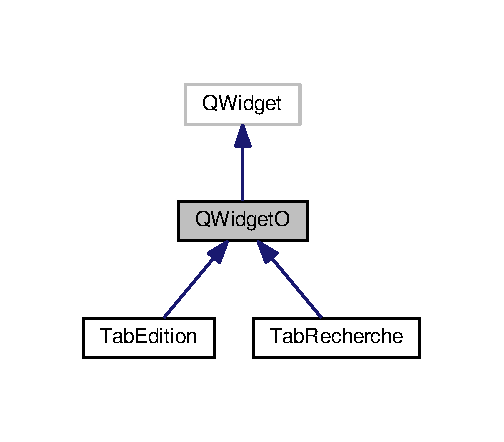
\includegraphics[width=242pt]{class_q_widget_o__inherit__graph}
\end{center}
\end{figure}


Graphe de collaboration de Q\+WidgetO\+:\nopagebreak
\begin{figure}[H]
\begin{center}
\leavevmode
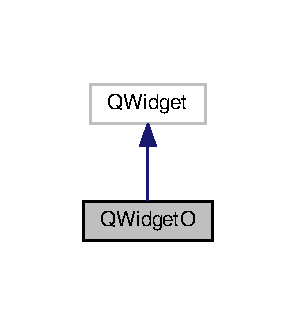
\includegraphics[width=142pt]{class_q_widget_o__coll__graph}
\end{center}
\end{figure}
\subsection*{Fonctions membres publiques}
\begin{DoxyCompactItemize}
\item 
\hyperlink{class_q_widget_o_a723ec63b442b10b2df002d9a007243f7}{Q\+WidgetO} (Q\+Widget $\ast$parent=0)
\begin{DoxyCompactList}\small\item\em Constructeur, crée un objet \hyperlink{class_q_widget_o}{Q\+WidgetO}. \end{DoxyCompactList}\item 
virtual void \hyperlink{class_q_widget_o_a39e3b81efd4553a71de86922ad683c40}{initialisation\+Buttons} ()=0\hypertarget{class_q_widget_o_a39e3b81efd4553a71de86922ad683c40}{}\label{class_q_widget_o_a39e3b81efd4553a71de86922ad683c40}

\begin{DoxyCompactList}\small\item\em procédure virtual permettant d\textquotesingle{}initialiser les buttons du widget \end{DoxyCompactList}\item 
virtual void \hyperlink{class_q_widget_o_a917af7ef0578b09dc8d60f1101ea14a7}{sup} (Q\+String name)=0
\begin{DoxyCompactList}\small\item\em procédure virtual de suppression du widget \end{DoxyCompactList}\end{DoxyCompactItemize}


\subsection{Description détaillée}
Classe permettant de redéfinir la classe Q\+Widget. 

\subsection{Documentation des constructeurs et destructeur}
\index{Q\+WidgetO@{Q\+WidgetO}!Q\+WidgetO@{Q\+WidgetO}}
\index{Q\+WidgetO@{Q\+WidgetO}!Q\+WidgetO@{Q\+WidgetO}}
\subsubsection[{\texorpdfstring{Q\+Widget\+O(\+Q\+Widget $\ast$parent=0)}{QWidgetO(QWidget *parent=0)}}]{\setlength{\rightskip}{0pt plus 5cm}Q\+Widget\+O\+::\+Q\+WidgetO (
\begin{DoxyParamCaption}
\item[{Q\+Widget $\ast$}]{parent = {\ttfamily 0}}
\end{DoxyParamCaption}
)\hspace{0.3cm}{\ttfamily [inline]}}\hypertarget{class_q_widget_o_a723ec63b442b10b2df002d9a007243f7}{}\label{class_q_widget_o_a723ec63b442b10b2df002d9a007243f7}


Constructeur, crée un objet \hyperlink{class_q_widget_o}{Q\+WidgetO}. 


\begin{DoxyParams}{Paramètres}
{\em Q\+Widget$\ast$,parent} & = 0 \\
\hline
\end{DoxyParams}


\subsection{Documentation des fonctions membres}
\index{Q\+WidgetO@{Q\+WidgetO}!sup@{sup}}
\index{sup@{sup}!Q\+WidgetO@{Q\+WidgetO}}
\subsubsection[{\texorpdfstring{sup(\+Q\+String name)=0}{sup(QString name)=0}}]{\setlength{\rightskip}{0pt plus 5cm}virtual void Q\+Widget\+O\+::sup (
\begin{DoxyParamCaption}
\item[{Q\+String}]{name}
\end{DoxyParamCaption}
)\hspace{0.3cm}{\ttfamily [pure virtual]}}\hypertarget{class_q_widget_o_a917af7ef0578b09dc8d60f1101ea14a7}{}\label{class_q_widget_o_a917af7ef0578b09dc8d60f1101ea14a7}


procédure virtual de suppression du widget 


\begin{DoxyParams}{Paramètres}
{\em Q\+String,name} & \\
\hline
\end{DoxyParams}


Implémenté dans \hyperlink{class_tab_edition_a844a8c4c5554d991957682ea9060cc59}{Tab\+Edition}, et \hyperlink{class_tab_recherche_a81618866cd661b7f4f2578ca79ae47f7}{Tab\+Recherche}.



La documentation de cette classe a été générée à partir du fichier suivant \+:\begin{DoxyCompactItemize}
\item 
Headers/\hyperlink{_q_widget_o_8h}{Q\+Widget\+O.\+h}\end{DoxyCompactItemize}

\hypertarget{class_style}{}\section{Référence de la classe Style}
\label{class_style}\index{Style@{Style}}


Classe permettant de définir la classe \hyperlink{class_style}{Style}.  




{\ttfamily \#include $<$Style.\+h$>$}

\subsection*{Fonctions membres publiques statiques}
\begin{DoxyCompactItemize}
\item 
static void \hyperlink{class_style_adee3a7fb2fab8c61cb5f6ebbcb44bfab}{set\+Style} (Q\+Push\+Button $\ast$button, int version)
\begin{DoxyCompactList}\small\item\em procédure permettant d\textquotesingle{}attribuer un style au boutton en fonction de la version choisis \end{DoxyCompactList}\end{DoxyCompactItemize}


\subsection{Description détaillée}
Classe permettant de définir la classe \hyperlink{class_style}{Style}. 

\subsection{Documentation des fonctions membres}
\index{Style@{Style}!set\+Style@{set\+Style}}
\index{set\+Style@{set\+Style}!Style@{Style}}
\subsubsection[{\texorpdfstring{set\+Style(\+Q\+Push\+Button $\ast$button, int version)}{setStyle(QPushButton *button, int version)}}]{\setlength{\rightskip}{0pt plus 5cm}void Style\+::set\+Style (
\begin{DoxyParamCaption}
\item[{Q\+Push\+Button $\ast$}]{button, }
\item[{int}]{version}
\end{DoxyParamCaption}
)\hspace{0.3cm}{\ttfamily [static]}}\hypertarget{class_style_adee3a7fb2fab8c61cb5f6ebbcb44bfab}{}\label{class_style_adee3a7fb2fab8c61cb5f6ebbcb44bfab}


procédure permettant d\textquotesingle{}attribuer un style au boutton en fonction de la version choisis 


\begin{DoxyParams}{Paramètres}
{\em Q\+Push\+Button$\ast$,button} & \\
\hline
{\em int,version} & \\
\hline
\end{DoxyParams}


La documentation de cette classe a été générée à partir des fichiers suivants \+:\begin{DoxyCompactItemize}
\item 
Headers/\hyperlink{_style_8h}{Style.\+h}\item 
Sources/\hyperlink{_style_8cpp}{Style.\+cpp}\end{DoxyCompactItemize}

\hypertarget{class_tab_edition}{}\section{Référence de la classe Tab\+Edition}
\label{class_tab_edition}\index{Tab\+Edition@{Tab\+Edition}}


Classe permettant de définir la classe \hyperlink{class_tab_edition}{Tab\+Edition}.  




{\ttfamily \#include $<$Tab\+Edition.\+h$>$}



Graphe d\textquotesingle{}héritage de Tab\+Edition\+:\nopagebreak
\begin{figure}[H]
\begin{center}
\leavevmode
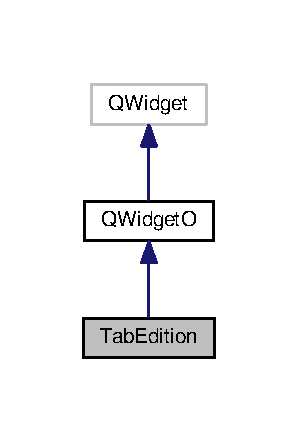
\includegraphics[width=143pt]{class_tab_edition__inherit__graph}
\end{center}
\end{figure}


Graphe de collaboration de Tab\+Edition\+:\nopagebreak
\begin{figure}[H]
\begin{center}
\leavevmode
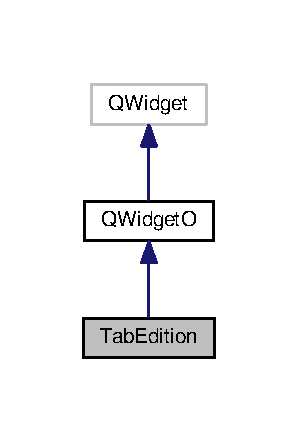
\includegraphics[width=143pt]{class_tab_edition__coll__graph}
\end{center}
\end{figure}
\subsection*{Connecteurs publics}
\begin{DoxyCompactItemize}
\item 
void \hyperlink{class_tab_edition_ae7affcb0acaf7fafdcc5586804907aed}{message\+Aide} ()\hypertarget{class_tab_edition_ae7affcb0acaf7fafdcc5586804907aed}{}\label{class_tab_edition_ae7affcb0acaf7fafdcc5586804907aed}

\begin{DoxyCompactList}\small\item\em procédure S\+L\+OT publique permettant d\textquotesingle{}afficher une pop-\/up d\textquotesingle{}aide edition \end{DoxyCompactList}\end{DoxyCompactItemize}
\subsection*{Fonctions membres publiques}
\begin{DoxyCompactItemize}
\item 
\hyperlink{class_tab_edition_ad02a3fd1d5aede64426945dc7e157a68}{Tab\+Edition} (\hyperlink{class_tags}{Tags} $\ast$tags, Q\+Widget $\ast$parent=0)
\begin{DoxyCompactList}\small\item\em Constructeur, crée un objet \hyperlink{class_tab_edition}{Tab\+Edition}. \end{DoxyCompactList}\item 
void \hyperlink{class_tab_edition_a2730367dae1f80a45875acb579b6f93e}{initialisation\+Buttons} ()\hypertarget{class_tab_edition_a2730367dae1f80a45875acb579b6f93e}{}\label{class_tab_edition_a2730367dae1f80a45875acb579b6f93e}

\begin{DoxyCompactList}\small\item\em procédure permettant d\textquotesingle{}initialiser les buttons du widget \end{DoxyCompactList}\item 
void \hyperlink{class_tab_edition_a9be046c1366dbee5f88becd6e02fe413}{initialisation\+Buttons\+List} ()\hypertarget{class_tab_edition_a9be046c1366dbee5f88becd6e02fe413}{}\label{class_tab_edition_a9be046c1366dbee5f88becd6e02fe413}

\begin{DoxyCompactList}\small\item\em procédure permettant d\textquotesingle{}initialiser les buttons des tags \end{DoxyCompactList}\item 
void \hyperlink{class_tab_edition_a9c8e4c8d033c7c0d5b4e1a37cb47d0f3}{clear\+Selected} ()\hypertarget{class_tab_edition_a9c8e4c8d033c7c0d5b4e1a37cb47d0f3}{}\label{class_tab_edition_a9c8e4c8d033c7c0d5b4e1a37cb47d0f3}

\begin{DoxyCompactList}\small\item\em procédure permettant de vider les listes de selection \end{DoxyCompactList}\item 
void \hyperlink{class_tab_edition_a844a8c4c5554d991957682ea9060cc59}{sup} (Q\+String name)
\begin{DoxyCompactList}\small\item\em procédure permettant de supprimer un tag de sa liste \end{DoxyCompactList}\item 
\hyperlink{class_tab_edition_ac7c6c640977a8c3273ee816762972f40}{$\sim$\+Tab\+Edition} ()\hypertarget{class_tab_edition_ac7c6c640977a8c3273ee816762972f40}{}\label{class_tab_edition_ac7c6c640977a8c3273ee816762972f40}

\begin{DoxyCompactList}\small\item\em Destructeur de \hyperlink{class_tab_edition}{Tab\+Edition}. \end{DoxyCompactList}\end{DoxyCompactItemize}


\subsection{Description détaillée}
Classe permettant de définir la classe \hyperlink{class_tab_edition}{Tab\+Edition}. 

\subsection{Documentation des constructeurs et destructeur}
\index{Tab\+Edition@{Tab\+Edition}!Tab\+Edition@{Tab\+Edition}}
\index{Tab\+Edition@{Tab\+Edition}!Tab\+Edition@{Tab\+Edition}}
\subsubsection[{\texorpdfstring{Tab\+Edition(\+Tags $\ast$tags, Q\+Widget $\ast$parent=0)}{TabEdition(Tags *tags, QWidget *parent=0)}}]{\setlength{\rightskip}{0pt plus 5cm}Tab\+Edition\+::\+Tab\+Edition (
\begin{DoxyParamCaption}
\item[{{\bf Tags} $\ast$}]{tags, }
\item[{Q\+Widget $\ast$}]{parent = {\ttfamily 0}}
\end{DoxyParamCaption}
)}\hypertarget{class_tab_edition_ad02a3fd1d5aede64426945dc7e157a68}{}\label{class_tab_edition_ad02a3fd1d5aede64426945dc7e157a68}


Constructeur, crée un objet \hyperlink{class_tab_edition}{Tab\+Edition}. 


\begin{DoxyParams}{Paramètres}
{\em Tags$\ast$,tags} & \\
\hline
{\em Q\+Widget$\ast$,parent} & = 0 \\
\hline
\end{DoxyParams}


\subsection{Documentation des fonctions membres}
\index{Tab\+Edition@{Tab\+Edition}!sup@{sup}}
\index{sup@{sup}!Tab\+Edition@{Tab\+Edition}}
\subsubsection[{\texorpdfstring{sup(\+Q\+String name)}{sup(QString name)}}]{\setlength{\rightskip}{0pt plus 5cm}void Tab\+Edition\+::sup (
\begin{DoxyParamCaption}
\item[{Q\+String}]{name}
\end{DoxyParamCaption}
)\hspace{0.3cm}{\ttfamily [virtual]}}\hypertarget{class_tab_edition_a844a8c4c5554d991957682ea9060cc59}{}\label{class_tab_edition_a844a8c4c5554d991957682ea9060cc59}


procédure permettant de supprimer un tag de sa liste 


\begin{DoxyParams}{Paramètres}
{\em Q\+String,name} & \\
\hline
\end{DoxyParams}


Implémente \hyperlink{class_q_widget_o_a917af7ef0578b09dc8d60f1101ea14a7}{Q\+WidgetO}.



La documentation de cette classe a été générée à partir des fichiers suivants \+:\begin{DoxyCompactItemize}
\item 
Headers/\hyperlink{_tab_edition_8h}{Tab\+Edition.\+h}\item 
Sources/\hyperlink{_tab_edition_8cpp}{Tab\+Edition.\+cpp}\end{DoxyCompactItemize}

\hypertarget{class_tab_recherche}{}\section{Référence de la classe Tab\+Recherche}
\label{class_tab_recherche}\index{Tab\+Recherche@{Tab\+Recherche}}


Classe permettant de définir la classe \hyperlink{class_tab_recherche}{Tab\+Recherche}.  




{\ttfamily \#include $<$Tab\+Recherche.\+h$>$}



Graphe d\textquotesingle{}héritage de Tab\+Recherche\+:\nopagebreak
\begin{figure}[H]
\begin{center}
\leavevmode
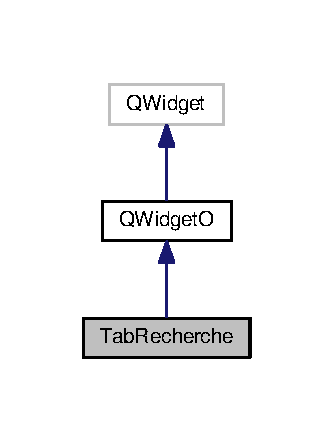
\includegraphics[width=160pt]{class_tab_recherche__inherit__graph}
\end{center}
\end{figure}


Graphe de collaboration de Tab\+Recherche\+:\nopagebreak
\begin{figure}[H]
\begin{center}
\leavevmode
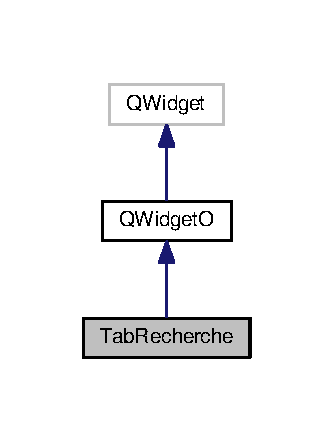
\includegraphics[width=160pt]{class_tab_recherche__coll__graph}
\end{center}
\end{figure}
\subsection*{Connecteurs publics}
\begin{DoxyCompactItemize}
\item 
void \hyperlink{class_tab_recherche_a3eae26f6020103f44a0ac5e27a35f0e1}{message\+Aide} ()\hypertarget{class_tab_recherche_a3eae26f6020103f44a0ac5e27a35f0e1}{}\label{class_tab_recherche_a3eae26f6020103f44a0ac5e27a35f0e1}

\begin{DoxyCompactList}\small\item\em procédure S\+L\+OT publique permettant d\textquotesingle{}afficher une pop-\/up d\textquotesingle{}aide edition \end{DoxyCompactList}\end{DoxyCompactItemize}
\subsection*{Fonctions membres publiques}
\begin{DoxyCompactItemize}
\item 
\hyperlink{class_tab_recherche_a97ce35f523049227c55bf651303bb4de}{Tab\+Recherche} (\hyperlink{class_tags}{Tags} $\ast$tags, Q\+Widget $\ast$parent=0)
\begin{DoxyCompactList}\small\item\em Constructeur, crée un objet \hyperlink{class_tab_recherche}{Tab\+Recherche}. \end{DoxyCompactList}\item 
void \hyperlink{class_tab_recherche_acf8a4104c762f41a3750d24473d17092}{initialisation\+Buttons} ()\hypertarget{class_tab_recherche_acf8a4104c762f41a3750d24473d17092}{}\label{class_tab_recherche_acf8a4104c762f41a3750d24473d17092}

\begin{DoxyCompactList}\small\item\em procédure permettant d\textquotesingle{}initialiser les buttons du widget \end{DoxyCompactList}\item 
void \hyperlink{class_tab_recherche_a81618866cd661b7f4f2578ca79ae47f7}{sup} (Q\+String name)
\begin{DoxyCompactList}\small\item\em procédure permettant de supprimer un tag \end{DoxyCompactList}\item 
\hyperlink{class_tab_recherche_ab39802929110947b784fb0bc420f69a5}{$\sim$\+Tab\+Recherche} ()\hypertarget{class_tab_recherche_ab39802929110947b784fb0bc420f69a5}{}\label{class_tab_recherche_ab39802929110947b784fb0bc420f69a5}

\begin{DoxyCompactList}\small\item\em Destructeur de \hyperlink{class_tab_recherche}{Tab\+Recherche}. \end{DoxyCompactList}\end{DoxyCompactItemize}


\subsection{Description détaillée}
Classe permettant de définir la classe \hyperlink{class_tab_recherche}{Tab\+Recherche}. 

\subsection{Documentation des constructeurs et destructeur}
\index{Tab\+Recherche@{Tab\+Recherche}!Tab\+Recherche@{Tab\+Recherche}}
\index{Tab\+Recherche@{Tab\+Recherche}!Tab\+Recherche@{Tab\+Recherche}}
\subsubsection[{\texorpdfstring{Tab\+Recherche(\+Tags $\ast$tags, Q\+Widget $\ast$parent=0)}{TabRecherche(Tags *tags, QWidget *parent=0)}}]{\setlength{\rightskip}{0pt plus 5cm}Tab\+Recherche\+::\+Tab\+Recherche (
\begin{DoxyParamCaption}
\item[{{\bf Tags} $\ast$}]{tags, }
\item[{Q\+Widget $\ast$}]{parent = {\ttfamily 0}}
\end{DoxyParamCaption}
)}\hypertarget{class_tab_recherche_a97ce35f523049227c55bf651303bb4de}{}\label{class_tab_recherche_a97ce35f523049227c55bf651303bb4de}


Constructeur, crée un objet \hyperlink{class_tab_recherche}{Tab\+Recherche}. 


\begin{DoxyParams}{Paramètres}
{\em Tags$\ast$,tags} & \\
\hline
{\em Q\+Widget$\ast$,parent} & = 0 \\
\hline
\end{DoxyParams}


\subsection{Documentation des fonctions membres}
\index{Tab\+Recherche@{Tab\+Recherche}!sup@{sup}}
\index{sup@{sup}!Tab\+Recherche@{Tab\+Recherche}}
\subsubsection[{\texorpdfstring{sup(\+Q\+String name)}{sup(QString name)}}]{\setlength{\rightskip}{0pt plus 5cm}void Tab\+Recherche\+::sup (
\begin{DoxyParamCaption}
\item[{Q\+String}]{name}
\end{DoxyParamCaption}
)\hspace{0.3cm}{\ttfamily [virtual]}}\hypertarget{class_tab_recherche_a81618866cd661b7f4f2578ca79ae47f7}{}\label{class_tab_recherche_a81618866cd661b7f4f2578ca79ae47f7}


procédure permettant de supprimer un tag 


\begin{DoxyParams}{Paramètres}
{\em Q\+String,name} & \\
\hline
\end{DoxyParams}


Implémente \hyperlink{class_q_widget_o_a917af7ef0578b09dc8d60f1101ea14a7}{Q\+WidgetO}.



La documentation de cette classe a été générée à partir des fichiers suivants \+:\begin{DoxyCompactItemize}
\item 
Headers/\hyperlink{_tab_recherche_8h}{Tab\+Recherche.\+h}\item 
Sources/\hyperlink{_tab_recherche_8cpp}{Tab\+Recherche.\+cpp}\end{DoxyCompactItemize}

\hypertarget{class_tag}{}\section{Référence de la classe Tag}
\label{class_tag}\index{Tag@{Tag}}


Classe permettant de représenter un tag (chaque tag possède un nom et une liste de chemin qui lui ont été associé)  




{\ttfamily \#include $<$Tag.\+h$>$}

\subsection*{Fonctions membres publiques}
\begin{DoxyCompactItemize}
\item 
\hyperlink{class_tag_a1dc354cd81ef646b6d1a88f8d792acab}{Tag} (Q\+String name)
\begin{DoxyCompactList}\small\item\em Constructeur, crée un objet \hyperlink{class_tag}{Tag} avec un nom mis en paramètre. \end{DoxyCompactList}\item 
Q\+List$<$ Q\+String $>$ \hyperlink{class_tag_ae59f1dfea121805d056982fb4fc256a3}{get\+List\+Ways} ()
\begin{DoxyCompactList}\small\item\em Getter de l\textquotesingle{}attribut List\+Ways. \end{DoxyCompactList}\item 
Q\+String \hyperlink{class_tag_a0aa1b1560628e5f2ba0ac2782fe1f6a2}{get\+Name} ()
\begin{DoxyCompactList}\small\item\em Getter de l\textquotesingle{}attribut Name. \end{DoxyCompactList}\item 
void \hyperlink{class_tag_a6e01670a53e191a0aa8dbd19e553ae17}{Add\+Way} (Q\+String way, bool write)
\begin{DoxyCompactList}\small\item\em procédure permettant d\textquotesingle{}ajouter une association(chemin) dans la List\+Ways et avec une ecriture dans le fichier \end{DoxyCompactList}\item 
bool \hyperlink{class_tag_aef29fdee7946c77e1458344b6f5caae0}{is} (Q\+String name)
\begin{DoxyCompactList}\small\item\em fonction retournant le bool si le tag possède le même nom \end{DoxyCompactList}\item 
void \hyperlink{class_tag_a78f2b199c0dfddf91155c2c310d7b9b7}{initialiser\+Tag\+Files} ()\hypertarget{class_tag_a78f2b199c0dfddf91155c2c310d7b9b7}{}\label{class_tag_a78f2b199c0dfddf91155c2c310d7b9b7}

\begin{DoxyCompactList}\small\item\em procédure permettant d\textquotesingle{}initialiser List\+Ways avec son fichier de config \end{DoxyCompactList}\item 
bool \hyperlink{class_tag_afc82c9681eb14d892879ddab2b4811c4}{tag\+Possedant} (Q\+String way)
\begin{DoxyCompactList}\small\item\em fonction retournant le bool si le tag possède cette association (chemin) \end{DoxyCompactList}\item 
void \hyperlink{class_tag_acc722c521a916ac500abd9dc7d887413}{sup\+Way} (Q\+String way)
\begin{DoxyCompactList}\small\item\em procédure permettant de supprimer une association(chemin) \end{DoxyCompactList}\item 
\hyperlink{class_tag_aa582ff83996a96e1c7e0fabe9350e166}{$\sim$\+Tag} ()\hypertarget{class_tag_aa582ff83996a96e1c7e0fabe9350e166}{}\label{class_tag_aa582ff83996a96e1c7e0fabe9350e166}

\begin{DoxyCompactList}\small\item\em Destructeur de \hyperlink{class_tag}{Tag}. \end{DoxyCompactList}\end{DoxyCompactItemize}


\subsection{Description détaillée}
Classe permettant de représenter un tag (chaque tag possède un nom et une liste de chemin qui lui ont été associé) 

\subsection{Documentation des constructeurs et destructeur}
\index{Tag@{Tag}!Tag@{Tag}}
\index{Tag@{Tag}!Tag@{Tag}}
\subsubsection[{\texorpdfstring{Tag(\+Q\+String name)}{Tag(QString name)}}]{\setlength{\rightskip}{0pt plus 5cm}Tag\+::\+Tag (
\begin{DoxyParamCaption}
\item[{Q\+String}]{name}
\end{DoxyParamCaption}
)}\hypertarget{class_tag_a1dc354cd81ef646b6d1a88f8d792acab}{}\label{class_tag_a1dc354cd81ef646b6d1a88f8d792acab}


Constructeur, crée un objet \hyperlink{class_tag}{Tag} avec un nom mis en paramètre. 


\begin{DoxyParams}{Paramètres}
{\em Q\+String,name} & \\
\hline
\end{DoxyParams}


\subsection{Documentation des fonctions membres}
\index{Tag@{Tag}!Add\+Way@{Add\+Way}}
\index{Add\+Way@{Add\+Way}!Tag@{Tag}}
\subsubsection[{\texorpdfstring{Add\+Way(\+Q\+String way, bool write)}{AddWay(QString way, bool write)}}]{\setlength{\rightskip}{0pt plus 5cm}void Tag\+::\+Add\+Way (
\begin{DoxyParamCaption}
\item[{Q\+String}]{way, }
\item[{bool}]{write}
\end{DoxyParamCaption}
)}\hypertarget{class_tag_a6e01670a53e191a0aa8dbd19e553ae17}{}\label{class_tag_a6e01670a53e191a0aa8dbd19e553ae17}


procédure permettant d\textquotesingle{}ajouter une association(chemin) dans la List\+Ways et avec une ecriture dans le fichier 


\begin{DoxyParams}{Paramètres}
{\em Q\+String} & way, bool write \\
\hline
\end{DoxyParams}
\index{Tag@{Tag}!get\+List\+Ways@{get\+List\+Ways}}
\index{get\+List\+Ways@{get\+List\+Ways}!Tag@{Tag}}
\subsubsection[{\texorpdfstring{get\+List\+Ways()}{getListWays()}}]{\setlength{\rightskip}{0pt plus 5cm}Q\+List$<$ Q\+String $>$ Tag\+::get\+List\+Ways (
\begin{DoxyParamCaption}
{}
\end{DoxyParamCaption}
)}\hypertarget{class_tag_ae59f1dfea121805d056982fb4fc256a3}{}\label{class_tag_ae59f1dfea121805d056982fb4fc256a3}


Getter de l\textquotesingle{}attribut List\+Ways. 

\begin{DoxyReturn}{Renvoie}
attribut List\+Ways 
\end{DoxyReturn}
\index{Tag@{Tag}!get\+Name@{get\+Name}}
\index{get\+Name@{get\+Name}!Tag@{Tag}}
\subsubsection[{\texorpdfstring{get\+Name()}{getName()}}]{\setlength{\rightskip}{0pt plus 5cm}Q\+String Tag\+::get\+Name (
\begin{DoxyParamCaption}
{}
\end{DoxyParamCaption}
)}\hypertarget{class_tag_a0aa1b1560628e5f2ba0ac2782fe1f6a2}{}\label{class_tag_a0aa1b1560628e5f2ba0ac2782fe1f6a2}


Getter de l\textquotesingle{}attribut Name. 

\begin{DoxyReturn}{Renvoie}
attribut Name 
\end{DoxyReturn}
\index{Tag@{Tag}!is@{is}}
\index{is@{is}!Tag@{Tag}}
\subsubsection[{\texorpdfstring{is(\+Q\+String name)}{is(QString name)}}]{\setlength{\rightskip}{0pt plus 5cm}bool Tag\+::is (
\begin{DoxyParamCaption}
\item[{Q\+String}]{name}
\end{DoxyParamCaption}
)}\hypertarget{class_tag_aef29fdee7946c77e1458344b6f5caae0}{}\label{class_tag_aef29fdee7946c77e1458344b6f5caae0}


fonction retournant le bool si le tag possède le même nom 


\begin{DoxyParams}{Paramètres}
{\em Q\+String} & name \\
\hline
\end{DoxyParams}
\index{Tag@{Tag}!sup\+Way@{sup\+Way}}
\index{sup\+Way@{sup\+Way}!Tag@{Tag}}
\subsubsection[{\texorpdfstring{sup\+Way(\+Q\+String way)}{supWay(QString way)}}]{\setlength{\rightskip}{0pt plus 5cm}void Tag\+::sup\+Way (
\begin{DoxyParamCaption}
\item[{Q\+String}]{way}
\end{DoxyParamCaption}
)}\hypertarget{class_tag_acc722c521a916ac500abd9dc7d887413}{}\label{class_tag_acc722c521a916ac500abd9dc7d887413}


procédure permettant de supprimer une association(chemin) 


\begin{DoxyParams}{Paramètres}
{\em Q\+String} & way \\
\hline
\end{DoxyParams}
\index{Tag@{Tag}!tag\+Possedant@{tag\+Possedant}}
\index{tag\+Possedant@{tag\+Possedant}!Tag@{Tag}}
\subsubsection[{\texorpdfstring{tag\+Possedant(\+Q\+String way)}{tagPossedant(QString way)}}]{\setlength{\rightskip}{0pt plus 5cm}bool Tag\+::tag\+Possedant (
\begin{DoxyParamCaption}
\item[{Q\+String}]{way}
\end{DoxyParamCaption}
)}\hypertarget{class_tag_afc82c9681eb14d892879ddab2b4811c4}{}\label{class_tag_afc82c9681eb14d892879ddab2b4811c4}


fonction retournant le bool si le tag possède cette association (chemin) 


\begin{DoxyParams}{Paramètres}
{\em Q\+String} & way \\
\hline
\end{DoxyParams}


La documentation de cette classe a été générée à partir des fichiers suivants \+:\begin{DoxyCompactItemize}
\item 
Headers/\hyperlink{_tag_8h}{Tag.\+h}\item 
Sources/Tag.\+cpp\end{DoxyCompactItemize}

\hypertarget{class_tags}{}\section{Référence de la classe Tags}
\label{class_tags}\index{Tags@{Tags}}


Classe permettant de lister les différents tags et possède un pointeur vers les deux modes.  




{\ttfamily \#include $<$Tags.\+h$>$}

\subsection*{Fonctions membres publiques}
\begin{DoxyCompactItemize}
\item 
\hyperlink{class_tags_a8d3045112662e0ace4b8bafb5a3e8f57}{Tags} ()\hypertarget{class_tags_a8d3045112662e0ace4b8bafb5a3e8f57}{}\label{class_tags_a8d3045112662e0ace4b8bafb5a3e8f57}

\begin{DoxyCompactList}\small\item\em Constructeur, crée un objet \hyperlink{class_tags}{Tags}. \end{DoxyCompactList}\item 
\hyperlink{class_q_widget_o}{Q\+WidgetO} $\ast$ \hyperlink{class_tags_ac7b0c253bbea81ebec2f17fd628b67e2}{get\+Tab\+Recherche} ()
\begin{DoxyCompactList}\small\item\em Getter de l\textquotesingle{}attribut \hyperlink{class_tab_recherche}{Tab\+Recherche}. \end{DoxyCompactList}\item 
\hyperlink{class_q_widget_o}{Q\+WidgetO} $\ast$ \hyperlink{class_tags_aea3b5ed347a1eb66f41fc84d0d174d45}{get\+Tab\+Edition} ()
\begin{DoxyCompactList}\small\item\em Getter de l\textquotesingle{}attribut \hyperlink{class_tab_edition}{Tab\+Edition}. \end{DoxyCompactList}\item 
Q\+List$<$ \hyperlink{class_tag}{Tag} $\ast$ $>$ \hyperlink{class_tags_aab1b32558374b97adde959c3822d804d}{get\+List\+Tags} ()
\begin{DoxyCompactList}\small\item\em Getter de l\textquotesingle{}attribut List\+Tags. \end{DoxyCompactList}\item 
\hyperlink{class_tag}{Tag} $\ast$ \hyperlink{class_tags_a8068c802b3da7261d9b271fa566d6de7}{get\+Tag} (Q\+String name\+Tag)
\begin{DoxyCompactList}\small\item\em Getter d\textquotesingle{}un pointeur de tag possèdant le même nom que celui mis en paramètre. \end{DoxyCompactList}\item 
void \hyperlink{class_tags_a57abf29a5ab4a089a7d8e6b55c1f508f}{set\+Q\+Widget\+Recherche} (\hyperlink{class_q_widget_o}{Q\+WidgetO} $\ast$\hyperlink{class_tab_recherche}{Tab\+Recherche})
\begin{DoxyCompactList}\small\item\em Setter de l\textquotesingle{}attribut \hyperlink{class_tab_recherche}{Tab\+Recherche}. \end{DoxyCompactList}\item 
void \hyperlink{class_tags_a62d0a0430258dc94fb6aa41bd5558b19}{set\+Q\+Widget\+Edition} (\hyperlink{class_q_widget_o}{Q\+WidgetO} $\ast$\hyperlink{class_tab_edition}{Tab\+Edition})
\begin{DoxyCompactList}\small\item\em Setter de l\textquotesingle{}attribut \hyperlink{class_tab_edition}{Tab\+Edition}. \end{DoxyCompactList}\item 
void \hyperlink{class_tags_a72f68c1babf29e2c5f1e49356dbe71ab}{supprimer\+Tag} (\hyperlink{class_tag}{Tag} $\ast$tag)
\begin{DoxyCompactList}\small\item\em Procédure permettant de supprimer un tag dans \hyperlink{class_tags}{Tags} et de modifier/supprimer les fichiers de configs respectifs. \end{DoxyCompactList}\item 
void \hyperlink{class_tags_ac595bd17429b50a9a4b35f993670b44b}{initialiser\+Tags\+Files} ()\hypertarget{class_tags_ac595bd17429b50a9a4b35f993670b44b}{}\label{class_tags_ac595bd17429b50a9a4b35f993670b44b}

\begin{DoxyCompactList}\small\item\em procédure permettant d\textquotesingle{}initialiser tous les tags avec le fichier de config \end{DoxyCompactList}\item 
void \hyperlink{class_tags_a837588d5b1fa060ecc1c4c37cedbbe16}{add\+\_\+tag} (Q\+String name, bool write)
\begin{DoxyCompactList}\small\item\em Procédure permettant d\textquotesingle{}ajouter un tag dans \hyperlink{class_tags}{Tags} et de modifier/ajouter les fichiers de configs respectifs avec ecriture ou non. \end{DoxyCompactList}\item 
\hyperlink{class_tags_a8fbc021de7f063e0a8f0dc79a8894083}{$\sim$\+Tags} ()\hypertarget{class_tags_a8fbc021de7f063e0a8f0dc79a8894083}{}\label{class_tags_a8fbc021de7f063e0a8f0dc79a8894083}

\begin{DoxyCompactList}\small\item\em Destructeur de \hyperlink{class_tags}{Tags}. \end{DoxyCompactList}\end{DoxyCompactItemize}


\subsection{Description détaillée}
Classe permettant de lister les différents tags et possède un pointeur vers les deux modes. 

\subsection{Documentation des fonctions membres}
\index{Tags@{Tags}!add\+\_\+tag@{add\+\_\+tag}}
\index{add\+\_\+tag@{add\+\_\+tag}!Tags@{Tags}}
\subsubsection[{\texorpdfstring{add\+\_\+tag(\+Q\+String name, bool write)}{add_tag(QString name, bool write)}}]{\setlength{\rightskip}{0pt plus 5cm}void Tags\+::add\+\_\+tag (
\begin{DoxyParamCaption}
\item[{Q\+String}]{name, }
\item[{bool}]{write}
\end{DoxyParamCaption}
)}\hypertarget{class_tags_a837588d5b1fa060ecc1c4c37cedbbe16}{}\label{class_tags_a837588d5b1fa060ecc1c4c37cedbbe16}


Procédure permettant d\textquotesingle{}ajouter un tag dans \hyperlink{class_tags}{Tags} et de modifier/ajouter les fichiers de configs respectifs avec ecriture ou non. 


\begin{DoxyParams}{Paramètres}
{\em Q\+String,name} & \\
\hline
{\em bool,write} & \\
\hline
\end{DoxyParams}
\index{Tags@{Tags}!get\+List\+Tags@{get\+List\+Tags}}
\index{get\+List\+Tags@{get\+List\+Tags}!Tags@{Tags}}
\subsubsection[{\texorpdfstring{get\+List\+Tags()}{getListTags()}}]{\setlength{\rightskip}{0pt plus 5cm}Q\+List$<$ {\bf Tag} $\ast$ $>$ Tags\+::get\+List\+Tags (
\begin{DoxyParamCaption}
{}
\end{DoxyParamCaption}
)}\hypertarget{class_tags_aab1b32558374b97adde959c3822d804d}{}\label{class_tags_aab1b32558374b97adde959c3822d804d}


Getter de l\textquotesingle{}attribut List\+Tags. 

\begin{DoxyReturn}{Renvoie}
attribut List\+Tags 
\end{DoxyReturn}
\index{Tags@{Tags}!get\+Tab\+Edition@{get\+Tab\+Edition}}
\index{get\+Tab\+Edition@{get\+Tab\+Edition}!Tags@{Tags}}
\subsubsection[{\texorpdfstring{get\+Tab\+Edition()}{getTabEdition()}}]{\setlength{\rightskip}{0pt plus 5cm}{\bf Q\+WidgetO} $\ast$ Tags\+::get\+Tab\+Edition (
\begin{DoxyParamCaption}
{}
\end{DoxyParamCaption}
)}\hypertarget{class_tags_aea3b5ed347a1eb66f41fc84d0d174d45}{}\label{class_tags_aea3b5ed347a1eb66f41fc84d0d174d45}


Getter de l\textquotesingle{}attribut \hyperlink{class_tab_edition}{Tab\+Edition}. 

\begin{DoxyReturn}{Renvoie}
attribut \hyperlink{class_tab_edition}{Tab\+Edition} 
\end{DoxyReturn}
\index{Tags@{Tags}!get\+Tab\+Recherche@{get\+Tab\+Recherche}}
\index{get\+Tab\+Recherche@{get\+Tab\+Recherche}!Tags@{Tags}}
\subsubsection[{\texorpdfstring{get\+Tab\+Recherche()}{getTabRecherche()}}]{\setlength{\rightskip}{0pt plus 5cm}{\bf Q\+WidgetO} $\ast$ Tags\+::get\+Tab\+Recherche (
\begin{DoxyParamCaption}
{}
\end{DoxyParamCaption}
)}\hypertarget{class_tags_ac7b0c253bbea81ebec2f17fd628b67e2}{}\label{class_tags_ac7b0c253bbea81ebec2f17fd628b67e2}


Getter de l\textquotesingle{}attribut \hyperlink{class_tab_recherche}{Tab\+Recherche}. 

\begin{DoxyReturn}{Renvoie}
attribut \hyperlink{class_tab_recherche}{Tab\+Recherche} 
\end{DoxyReturn}
\index{Tags@{Tags}!get\+Tag@{get\+Tag}}
\index{get\+Tag@{get\+Tag}!Tags@{Tags}}
\subsubsection[{\texorpdfstring{get\+Tag(\+Q\+String name\+Tag)}{getTag(QString nameTag)}}]{\setlength{\rightskip}{0pt plus 5cm}{\bf Tag} $\ast$ Tags\+::get\+Tag (
\begin{DoxyParamCaption}
\item[{Q\+String}]{name\+Tag}
\end{DoxyParamCaption}
)}\hypertarget{class_tags_a8068c802b3da7261d9b271fa566d6de7}{}\label{class_tags_a8068c802b3da7261d9b271fa566d6de7}


Getter d\textquotesingle{}un pointeur de tag possèdant le même nom que celui mis en paramètre. 


\begin{DoxyParams}{Paramètres}
{\em Q\+String,name\+Tag} & \\
\hline
\end{DoxyParams}
\begin{DoxyReturn}{Renvoie}
Tag$\ast$ 
\end{DoxyReturn}
\index{Tags@{Tags}!set\+Q\+Widget\+Edition@{set\+Q\+Widget\+Edition}}
\index{set\+Q\+Widget\+Edition@{set\+Q\+Widget\+Edition}!Tags@{Tags}}
\subsubsection[{\texorpdfstring{set\+Q\+Widget\+Edition(\+Q\+Widget\+O $\ast$\+Tab\+Edition)}{setQWidgetEdition(QWidgetO *TabEdition)}}]{\setlength{\rightskip}{0pt plus 5cm}void Tags\+::set\+Q\+Widget\+Edition (
\begin{DoxyParamCaption}
\item[{{\bf Q\+WidgetO} $\ast$}]{Tab\+Edition}
\end{DoxyParamCaption}
)}\hypertarget{class_tags_a62d0a0430258dc94fb6aa41bd5558b19}{}\label{class_tags_a62d0a0430258dc94fb6aa41bd5558b19}


Setter de l\textquotesingle{}attribut \hyperlink{class_tab_edition}{Tab\+Edition}. 


\begin{DoxyParams}{Paramètres}
{\em Q\+Widget\+O$\ast$,\hyperlink{class_tab_edition}{Tab\+Edition}} & \\
\hline
\end{DoxyParams}
\index{Tags@{Tags}!set\+Q\+Widget\+Recherche@{set\+Q\+Widget\+Recherche}}
\index{set\+Q\+Widget\+Recherche@{set\+Q\+Widget\+Recherche}!Tags@{Tags}}
\subsubsection[{\texorpdfstring{set\+Q\+Widget\+Recherche(\+Q\+Widget\+O $\ast$\+Tab\+Recherche)}{setQWidgetRecherche(QWidgetO *TabRecherche)}}]{\setlength{\rightskip}{0pt plus 5cm}void Tags\+::set\+Q\+Widget\+Recherche (
\begin{DoxyParamCaption}
\item[{{\bf Q\+WidgetO} $\ast$}]{Tab\+Recherche}
\end{DoxyParamCaption}
)}\hypertarget{class_tags_a57abf29a5ab4a089a7d8e6b55c1f508f}{}\label{class_tags_a57abf29a5ab4a089a7d8e6b55c1f508f}


Setter de l\textquotesingle{}attribut \hyperlink{class_tab_recherche}{Tab\+Recherche}. 


\begin{DoxyParams}{Paramètres}
{\em Q\+Widget\+O$\ast$,\hyperlink{class_tab_recherche}{Tab\+Recherche}} & \\
\hline
\end{DoxyParams}
\index{Tags@{Tags}!supprimer\+Tag@{supprimer\+Tag}}
\index{supprimer\+Tag@{supprimer\+Tag}!Tags@{Tags}}
\subsubsection[{\texorpdfstring{supprimer\+Tag(\+Tag $\ast$tag)}{supprimerTag(Tag *tag)}}]{\setlength{\rightskip}{0pt plus 5cm}void Tags\+::supprimer\+Tag (
\begin{DoxyParamCaption}
\item[{{\bf Tag} $\ast$}]{tag}
\end{DoxyParamCaption}
)}\hypertarget{class_tags_a72f68c1babf29e2c5f1e49356dbe71ab}{}\label{class_tags_a72f68c1babf29e2c5f1e49356dbe71ab}


Procédure permettant de supprimer un tag dans \hyperlink{class_tags}{Tags} et de modifier/supprimer les fichiers de configs respectifs. 


\begin{DoxyParams}{Paramètres}
{\em Tag$\ast$,tag} & \\
\hline
\end{DoxyParams}


La documentation de cette classe a été générée à partir des fichiers suivants \+:\begin{DoxyCompactItemize}
\item 
Headers/\hyperlink{_tags_8h}{Tags.\+h}\item 
Sources/\hyperlink{_tags_8cpp}{Tags.\+cpp}\end{DoxyCompactItemize}

\chapter{Documentation des fichiers}
\hypertarget{_my_view_8h}{}\section{Référence du fichier Headers/\+My\+View.h}
\label{_my_view_8h}\index{Headers/\+My\+View.\+h@{Headers/\+My\+View.\+h}}


Définition d\textquotesingle{}une classe de \hyperlink{class_my_view}{My\+View}.  


{\ttfamily \#include $<$Q\+Table\+View$>$}\\*
{\ttfamily \#include $<$Q\+Point$>$}\\*
Graphe des dépendances par inclusion de My\+View.\+h\+:\nopagebreak
\begin{figure}[H]
\begin{center}
\leavevmode
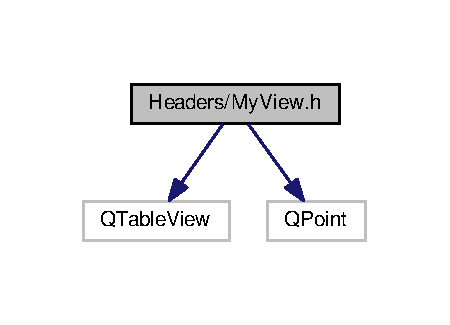
\includegraphics[width=216pt]{_my_view_8h__incl}
\end{center}
\end{figure}
Ce graphe montre quels fichiers incluent directement ou indirectement ce fichier \+:\nopagebreak
\begin{figure}[H]
\begin{center}
\leavevmode
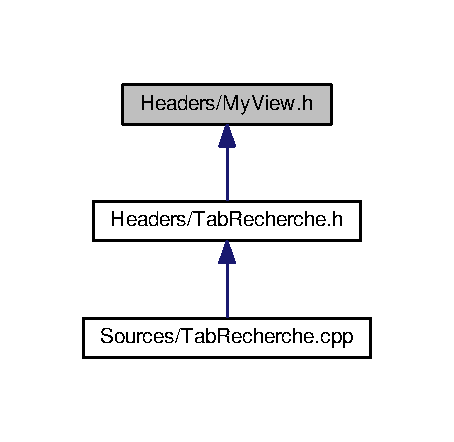
\includegraphics[width=218pt]{_my_view_8h__dep__incl}
\end{center}
\end{figure}
\subsection*{Classes}
\begin{DoxyCompactItemize}
\item 
class \hyperlink{class_my_view}{My\+View}
\begin{DoxyCompactList}\small\item\em Classe permettant de redéfinir la classe Q\+Table\+View. \end{DoxyCompactList}\end{DoxyCompactItemize}


\subsection{Description détaillée}
Définition d\textquotesingle{}une classe de \hyperlink{class_my_view}{My\+View}. 

\begin{DoxyAuthor}{Auteur}
G. Killian, P. Sullivan 
\end{DoxyAuthor}
\begin{DoxySince}{Depuis}
14/03/2017 
\end{DoxySince}

\hypertarget{_q_widget_o_8h}{}\section{Référence du fichier Headers/\+Q\+WidgetO.h}
\label{_q_widget_o_8h}\index{Headers/\+Q\+Widget\+O.\+h@{Headers/\+Q\+Widget\+O.\+h}}


Définition d\textquotesingle{}une classe de \hyperlink{class_q_widget_o}{Q\+WidgetO}.  


{\ttfamily \#include $<$Q\+Widget$>$}\\*
Graphe des dépendances par inclusion de Q\+Widget\+O.\+h\+:\nopagebreak
\begin{figure}[H]
\begin{center}
\leavevmode
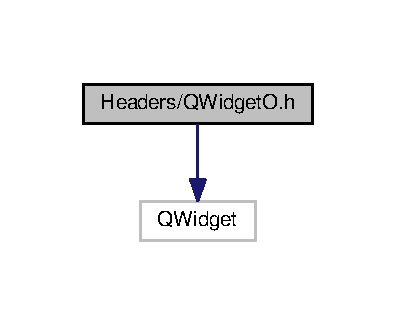
\includegraphics[width=190pt]{_q_widget_o_8h__incl}
\end{center}
\end{figure}
Ce graphe montre quels fichiers incluent directement ou indirectement ce fichier \+:\nopagebreak
\begin{figure}[H]
\begin{center}
\leavevmode
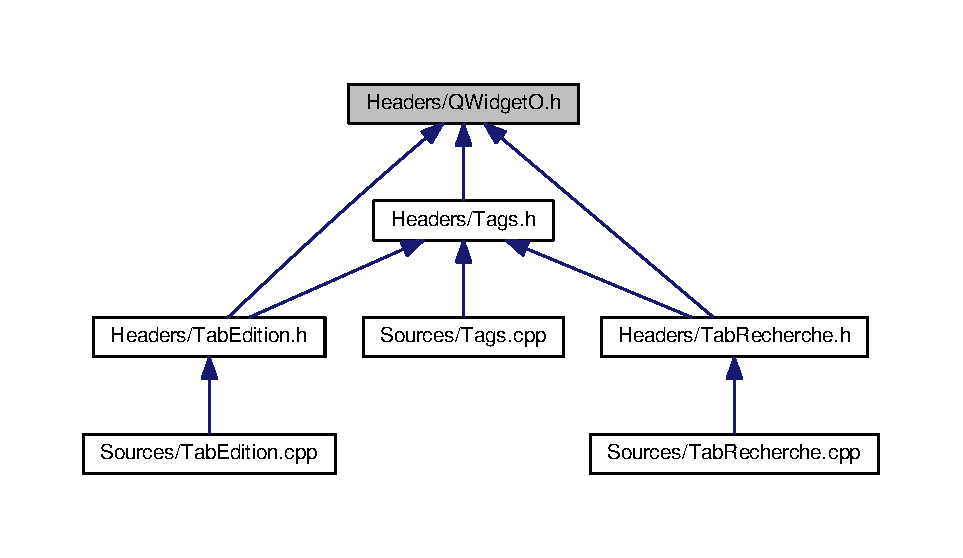
\includegraphics[width=350pt]{_q_widget_o_8h__dep__incl}
\end{center}
\end{figure}
\subsection*{Classes}
\begin{DoxyCompactItemize}
\item 
class \hyperlink{class_q_widget_o}{Q\+WidgetO}
\begin{DoxyCompactList}\small\item\em Classe permettant de redéfinir la classe Q\+Widget. \end{DoxyCompactList}\end{DoxyCompactItemize}


\subsection{Description détaillée}
Définition d\textquotesingle{}une classe de \hyperlink{class_q_widget_o}{Q\+WidgetO}. 

\begin{DoxyAuthor}{Auteur}
G. Killian, P. Sullivan 
\end{DoxyAuthor}
\begin{DoxySince}{Depuis}
14/03/2017 
\end{DoxySince}

\hypertarget{_style_8h}{}\section{Référence du fichier Headers/\+Style.h}
\label{_style_8h}\index{Headers/\+Style.\+h@{Headers/\+Style.\+h}}


Définition d\textquotesingle{}une classe de \hyperlink{class_style}{Style}.  


{\ttfamily \#include $<$Q\+Push\+Button$>$}\\*
Graphe des dépendances par inclusion de Style.\+h\+:\nopagebreak
\begin{figure}[H]
\begin{center}
\leavevmode
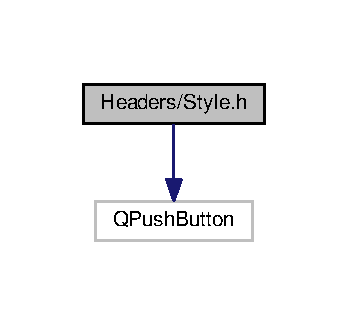
\includegraphics[width=167pt]{_style_8h__incl}
\end{center}
\end{figure}
Ce graphe montre quels fichiers incluent directement ou indirectement ce fichier \+:\nopagebreak
\begin{figure}[H]
\begin{center}
\leavevmode
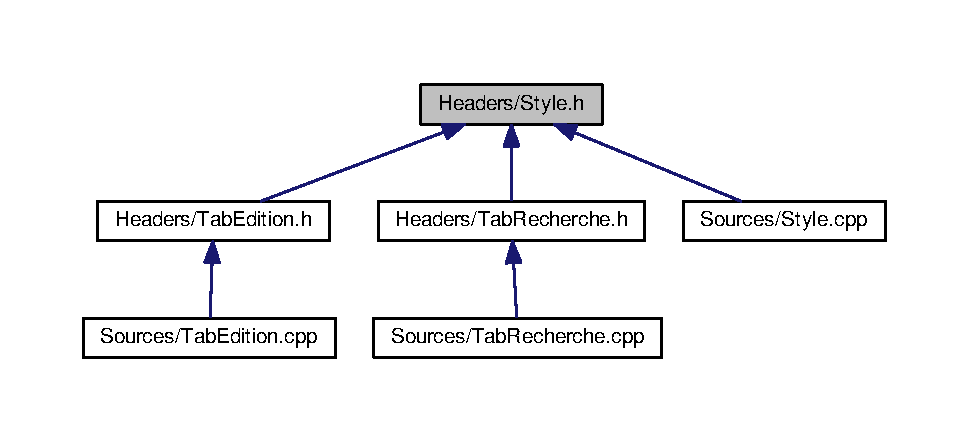
\includegraphics[width=350pt]{_style_8h__dep__incl}
\end{center}
\end{figure}
\subsection*{Classes}
\begin{DoxyCompactItemize}
\item 
class \hyperlink{class_style}{Style}
\begin{DoxyCompactList}\small\item\em Classe permettant de définir la classe \hyperlink{class_style}{Style}. \end{DoxyCompactList}\end{DoxyCompactItemize}


\subsection{Description détaillée}
Définition d\textquotesingle{}une classe de \hyperlink{class_style}{Style}. 

\begin{DoxyAuthor}{Auteur}
G. Killian, P. Sullivan 
\end{DoxyAuthor}
\begin{DoxySince}{Depuis}
14/03/2017 
\end{DoxySince}

\hypertarget{_tab_edition_8h}{}\section{Référence du fichier Headers/\+Tab\+Edition.h}
\label{_tab_edition_8h}\index{Headers/\+Tab\+Edition.\+h@{Headers/\+Tab\+Edition.\+h}}


Définition d\textquotesingle{}une classe de \hyperlink{class_tab_edition}{Tab\+Edition}.  


{\ttfamily \#include $<$Q\+Application$>$}\\*
{\ttfamily \#include $<$Q\+Push\+Button$>$}\\*
{\ttfamily \#include $<$Q\+Table\+Widget$>$}\\*
{\ttfamily \#include $<$Q\+H\+Box\+Layout$>$}\\*
{\ttfamily \#include $<$Q\+Message\+Box$>$}\\*
{\ttfamily \#include $<$Q\+Input\+Dialog$>$}\\*
{\ttfamily \#include $<$Q\+Tree\+View$>$}\\*
{\ttfamily \#include $<$string$>$}\\*
{\ttfamily \#include $<$Headers/\+Tags.\+h$>$}\\*
{\ttfamily \#include $<$Q\+File\+Dialog$>$}\\*
{\ttfamily \#include $<$Q\+File\+System\+Model$>$}\\*
{\ttfamily \#include $<$Q\+List\+View$>$}\\*
{\ttfamily \#include $<$Q\+Header\+View$>$}\\*
{\ttfamily \#include $<$Q\+List$>$}\\*
{\ttfamily \#include $<$Headers/\+Tag.\+h$>$}\\*
{\ttfamily \#include $<$Q\+Label$>$}\\*
{\ttfamily \#include $<$Headers/\+Q\+Widget\+O.\+h$>$}\\*
{\ttfamily \#include $<$Headers/\+Style.\+h$>$}\\*
{\ttfamily \#include $<$Headers/\+Q\+Push\+Button\+Plus.\+h$>$}\\*
{\ttfamily \#include $<$Q\+Menu\+Bar$>$}\\*
{\ttfamily \#include $<$Q\+Dir\+Model$>$}\\*
{\ttfamily \#include $<$Q\+Mouse\+Event$>$}\\*
Graphe des dépendances par inclusion de Tab\+Edition.\+h\+:\nopagebreak
\begin{figure}[H]
\begin{center}
\leavevmode
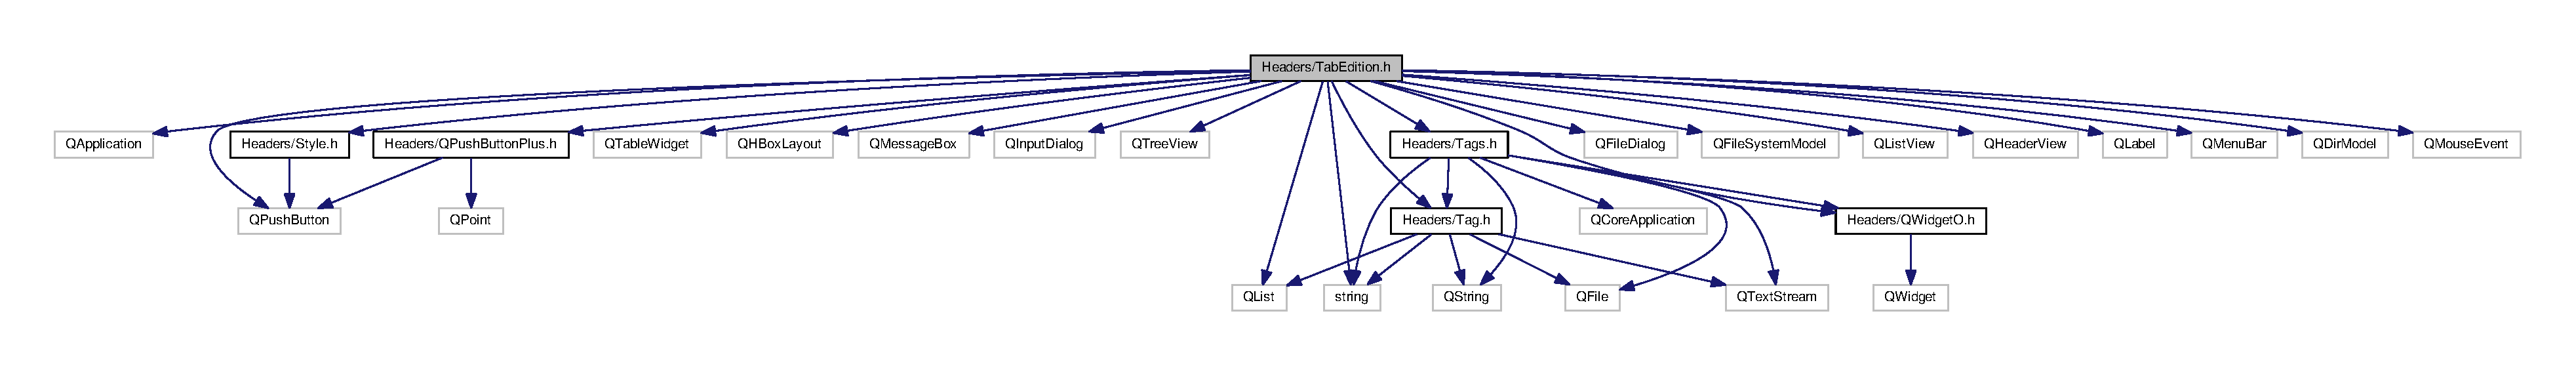
\includegraphics[width=350pt]{_tab_edition_8h__incl}
\end{center}
\end{figure}
Ce graphe montre quels fichiers incluent directement ou indirectement ce fichier \+:\nopagebreak
\begin{figure}[H]
\begin{center}
\leavevmode
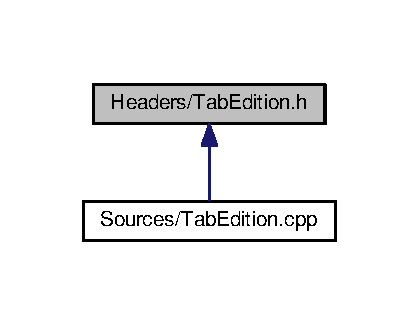
\includegraphics[width=201pt]{_tab_edition_8h__dep__incl}
\end{center}
\end{figure}
\subsection*{Classes}
\begin{DoxyCompactItemize}
\item 
class \hyperlink{class_tab_edition}{Tab\+Edition}
\begin{DoxyCompactList}\small\item\em Classe permettant de définir la classe \hyperlink{class_tab_edition}{Tab\+Edition}. \end{DoxyCompactList}\end{DoxyCompactItemize}


\subsection{Description détaillée}
Définition d\textquotesingle{}une classe de \hyperlink{class_tab_edition}{Tab\+Edition}. 

\begin{DoxyAuthor}{Auteur}
G. Killian, P. Sullivan 
\end{DoxyAuthor}
\begin{DoxySince}{Depuis}
14/03/2017 
\end{DoxySince}

\hypertarget{_tab_recherche_8h}{}\section{Référence du fichier Headers/\+Tab\+Recherche.h}
\label{_tab_recherche_8h}\index{Headers/\+Tab\+Recherche.\+h@{Headers/\+Tab\+Recherche.\+h}}


Définition d\textquotesingle{}une classe de \hyperlink{class_tab_recherche}{Tab\+Recherche}.  


{\ttfamily \#include $<$Q\+Application$>$}\\*
{\ttfamily \#include $<$Q\+Push\+Button$>$}\\*
{\ttfamily \#include $<$Q\+Table\+Widget$>$}\\*
{\ttfamily \#include $<$Q\+H\+Box\+Layout$>$}\\*
{\ttfamily \#include $<$Q\+Message\+Box$>$}\\*
{\ttfamily \#include $<$Headers/\+Tags.\+h$>$}\\*
{\ttfamily \#include $<$Headers/\+Q\+Widget\+O.\+h$>$}\\*
{\ttfamily \#include $<$Q\+Tree\+View$>$}\\*
{\ttfamily \#include $<$Q\+File\+System\+Model$>$}\\*
{\ttfamily \#include $<$Q\+Label$>$}\\*
{\ttfamily \#include $<$Q\+Standard\+Item\+Model$>$}\\*
{\ttfamily \#include $<$Headers/\+Q\+Push\+Button\+Plus.\+h$>$}\\*
{\ttfamily \#include $<$Q\+Menu\+Bar$>$}\\*
{\ttfamily \#include $<$Headers/\+Style.\+h$>$}\\*
{\ttfamily \#include $<$Headers/\+My\+View.\+h$>$}\\*
{\ttfamily \#include $<$Q\+File\+Info$>$}\\*
{\ttfamily \#include $<$Q\+Desktop\+Services$>$}\\*
{\ttfamily \#include $<$Q\+Url$>$}\\*
{\ttfamily \#include $<$Q\+Check\+Box$>$}\\*
{\ttfamily \#include $<$Q\+Tool\+Bar$>$}\\*
Graphe des dépendances par inclusion de Tab\+Recherche.\+h\+:\nopagebreak
\begin{figure}[H]
\begin{center}
\leavevmode
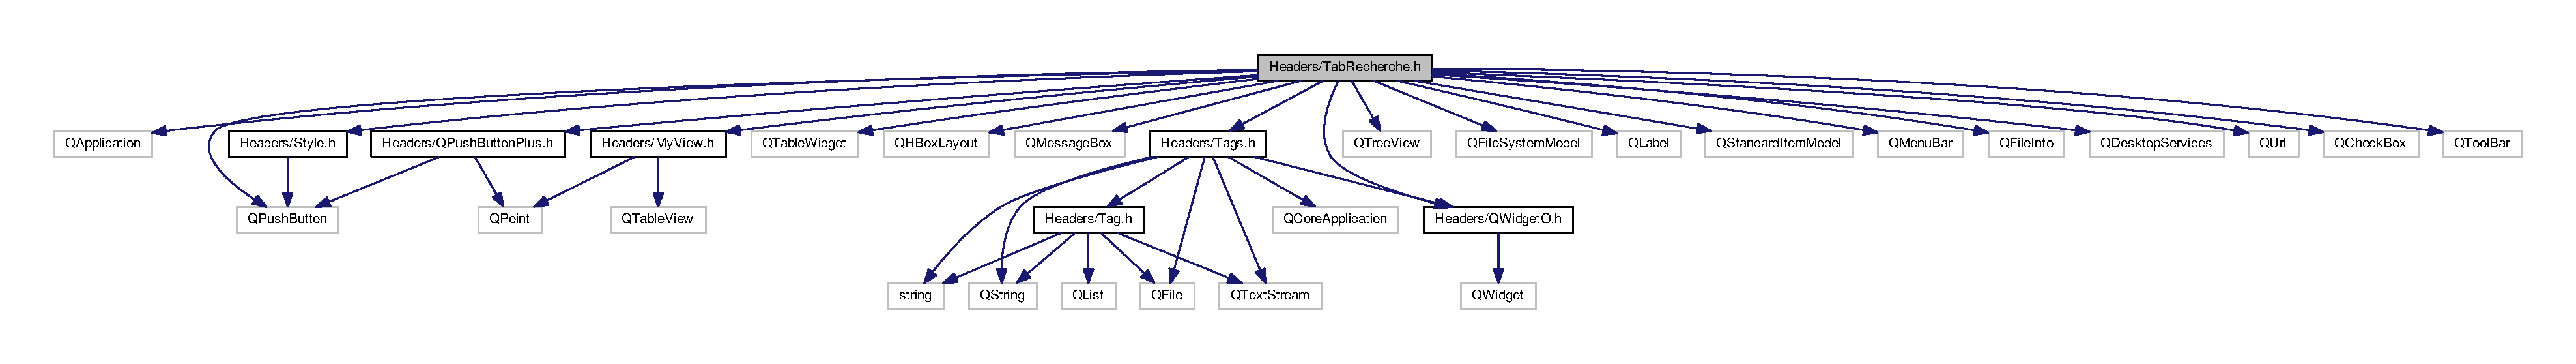
\includegraphics[width=350pt]{_tab_recherche_8h__incl}
\end{center}
\end{figure}
Ce graphe montre quels fichiers incluent directement ou indirectement ce fichier \+:\nopagebreak
\begin{figure}[H]
\begin{center}
\leavevmode
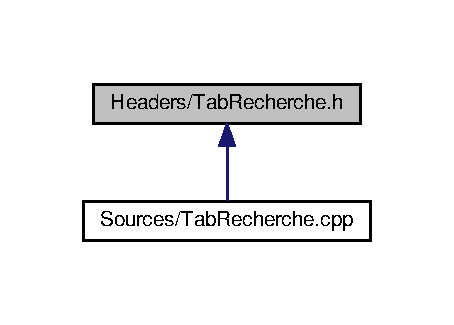
\includegraphics[width=218pt]{_tab_recherche_8h__dep__incl}
\end{center}
\end{figure}
\subsection*{Classes}
\begin{DoxyCompactItemize}
\item 
class \hyperlink{class_tab_recherche}{Tab\+Recherche}
\begin{DoxyCompactList}\small\item\em Classe permettant de définir la classe \hyperlink{class_tab_recherche}{Tab\+Recherche}. \end{DoxyCompactList}\end{DoxyCompactItemize}


\subsection{Description détaillée}
Définition d\textquotesingle{}une classe de \hyperlink{class_tab_recherche}{Tab\+Recherche}. 

\begin{DoxyAuthor}{Auteur}
G. Killian, P. Sullivan 
\end{DoxyAuthor}
\begin{DoxySince}{Depuis}
14/03/2017 
\end{DoxySince}

\hypertarget{_tag_8h}{}\section{Référence du fichier Headers/\+Tag.h}
\label{_tag_8h}\index{Headers/\+Tag.\+h@{Headers/\+Tag.\+h}}


Définition d\textquotesingle{}une classe de Tab.  


{\ttfamily \#include $<$string$>$}\\*
{\ttfamily \#include $<$Q\+String$>$}\\*
{\ttfamily \#include $<$Q\+List$>$}\\*
{\ttfamily \#include $<$Q\+File$>$}\\*
{\ttfamily \#include $<$Q\+Text\+Stream$>$}\\*
Graphe des dépendances par inclusion de Tag.\+h\+:\nopagebreak
\begin{figure}[H]
\begin{center}
\leavevmode
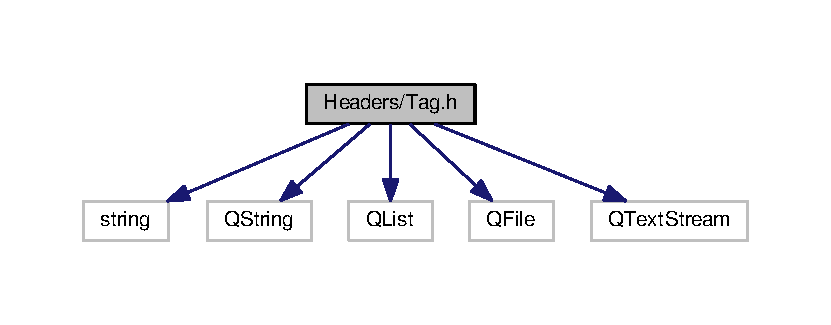
\includegraphics[width=350pt]{_tag_8h__incl}
\end{center}
\end{figure}
Ce graphe montre quels fichiers incluent directement ou indirectement ce fichier \+:\nopagebreak
\begin{figure}[H]
\begin{center}
\leavevmode
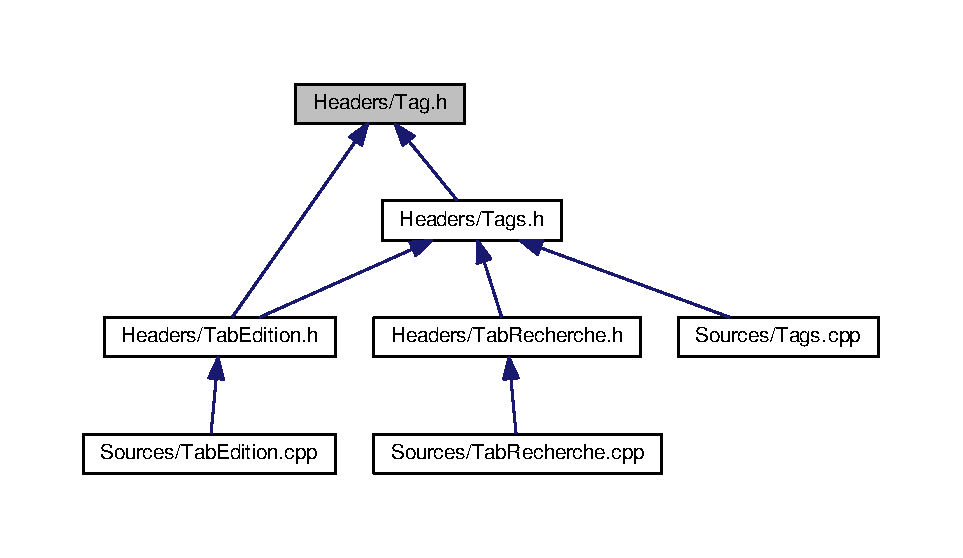
\includegraphics[width=350pt]{_tag_8h__dep__incl}
\end{center}
\end{figure}
\subsection*{Classes}
\begin{DoxyCompactItemize}
\item 
class \hyperlink{class_tag}{Tag}
\begin{DoxyCompactList}\small\item\em Classe permettant de représenter un tag (chaque tag possède un nom et une liste de chemin qui lui ont été associé) \end{DoxyCompactList}\end{DoxyCompactItemize}


\subsection{Description détaillée}
Définition d\textquotesingle{}une classe de Tab. 

\begin{DoxyAuthor}{Auteur}
G. Killian, P. Sullivan 
\end{DoxyAuthor}
\begin{DoxySince}{Depuis}
14/03/2017 
\end{DoxySince}

\hypertarget{_tags_8h}{}\section{Référence du fichier Headers/\+Tags.h}
\label{_tags_8h}\index{Headers/\+Tags.\+h@{Headers/\+Tags.\+h}}


Définition d\textquotesingle{}une classe de Tabs.  


{\ttfamily \#include $<$string$>$}\\*
{\ttfamily \#include $<$Q\+String$>$}\\*
{\ttfamily \#include $<$Headers/\+Tag.\+h$>$}\\*
{\ttfamily \#include $<$Headers/\+Q\+Widget\+O.\+h$>$}\\*
{\ttfamily \#include $<$Q\+File$>$}\\*
{\ttfamily \#include $<$Q\+Text\+Stream$>$}\\*
{\ttfamily \#include $<$Q\+Core\+Application$>$}\\*
Graphe des dépendances par inclusion de Tags.\+h\+:\nopagebreak
\begin{figure}[H]
\begin{center}
\leavevmode
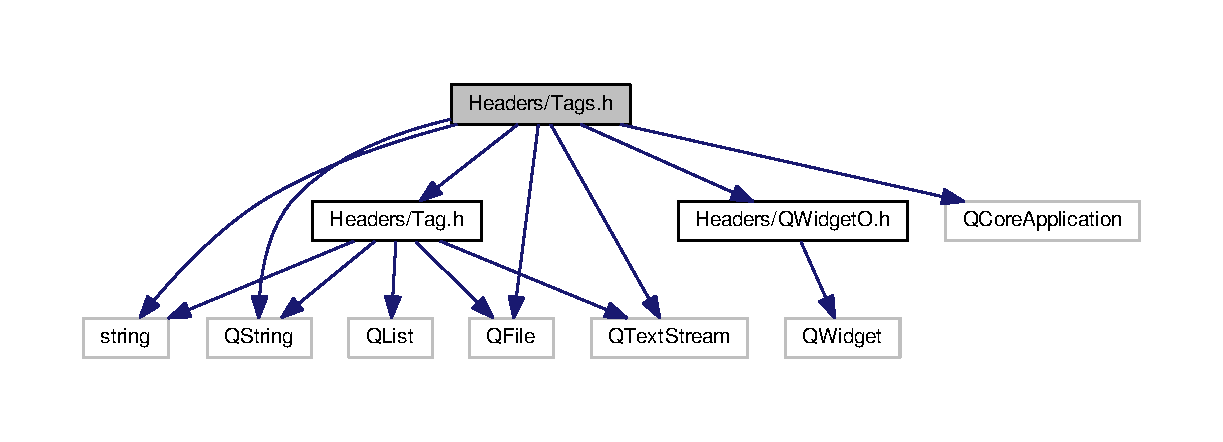
\includegraphics[width=350pt]{_tags_8h__incl}
\end{center}
\end{figure}
Ce graphe montre quels fichiers incluent directement ou indirectement ce fichier \+:\nopagebreak
\begin{figure}[H]
\begin{center}
\leavevmode
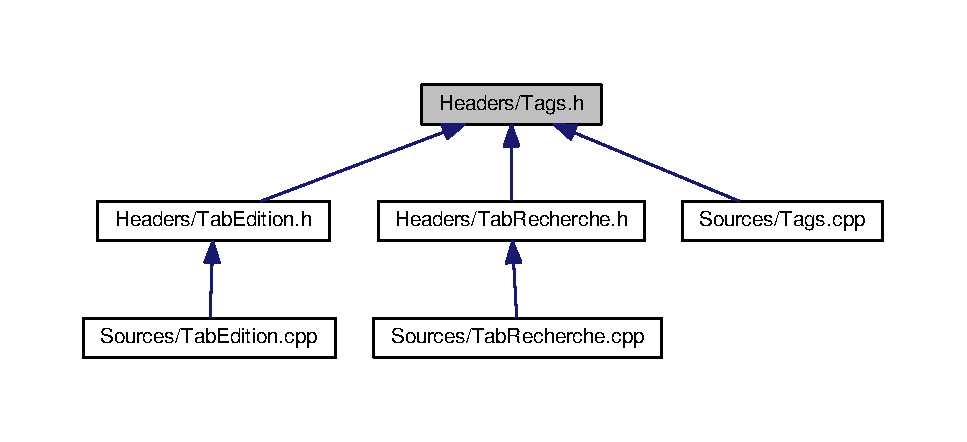
\includegraphics[width=350pt]{_tags_8h__dep__incl}
\end{center}
\end{figure}
\subsection*{Classes}
\begin{DoxyCompactItemize}
\item 
class \hyperlink{class_tags}{Tags}
\begin{DoxyCompactList}\small\item\em Classe permettant de lister les différents tags et possède un pointeur vers les deux modes. \end{DoxyCompactList}\end{DoxyCompactItemize}


\subsection{Description détaillée}
Définition d\textquotesingle{}une classe de Tabs. 

\begin{DoxyAuthor}{Auteur}
G. Killian, P. Sullivan 
\end{DoxyAuthor}
\begin{DoxySince}{Depuis}
14/03/2017 
\end{DoxySince}

\hypertarget{_q_push_button_plus_8cpp}{}\section{Référence du fichier Sources/\+Q\+Push\+Button\+Plus.cpp}
\label{_q_push_button_plus_8cpp}\index{Sources/\+Q\+Push\+Button\+Plus.\+cpp@{Sources/\+Q\+Push\+Button\+Plus.\+cpp}}


implémentation des méthodes de la classe \hyperlink{class_q_push_button_plus}{Q\+Push\+Button\+Plus}  


{\ttfamily \#include \char`\"{}Headers/\+Q\+Push\+Button\+Plus.\+h\char`\"{}}\\*
{\ttfamily \#include $<$Q\+Mouse\+Event$>$}\\*
Graphe des dépendances par inclusion de Q\+Push\+Button\+Plus.\+cpp\+:\nopagebreak
\begin{figure}[H]
\begin{center}
\leavevmode
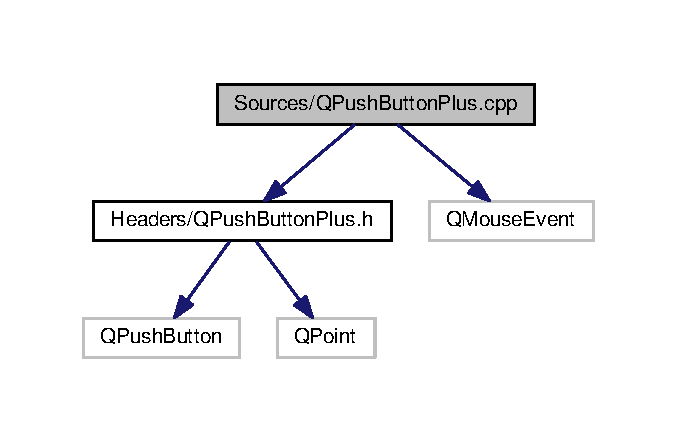
\includegraphics[width=325pt]{_q_push_button_plus_8cpp__incl}
\end{center}
\end{figure}


\subsection{Description détaillée}
implémentation des méthodes de la classe \hyperlink{class_q_push_button_plus}{Q\+Push\+Button\+Plus} 

\begin{DoxyAuthor}{Auteur}
G. Killian, P. Sullivan 
\end{DoxyAuthor}
\begin{DoxySince}{Depuis}
14/03/2017 
\end{DoxySince}

\hypertarget{_style_8cpp}{}\section{Référence du fichier Sources/\+Style.cpp}
\label{_style_8cpp}\index{Sources/\+Style.\+cpp@{Sources/\+Style.\+cpp}}


implémentation de la méthode de la classe \hyperlink{class_style}{Style}  


{\ttfamily \#include \char`\"{}Headers/\+Style.\+h\char`\"{}}\\*
Graphe des dépendances par inclusion de Style.\+cpp\+:\nopagebreak
\begin{figure}[H]
\begin{center}
\leavevmode
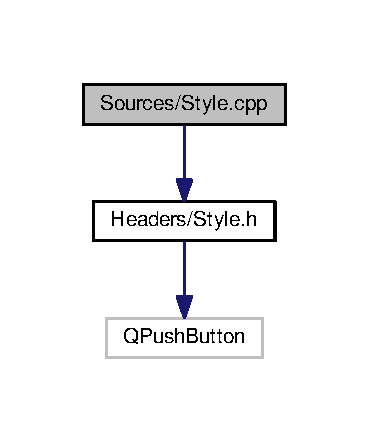
\includegraphics[width=177pt]{_style_8cpp__incl}
\end{center}
\end{figure}


\subsection{Description détaillée}
implémentation de la méthode de la classe \hyperlink{class_style}{Style} 

\begin{DoxyAuthor}{Auteur}
G. Killian, P. Sullivan 
\end{DoxyAuthor}
\begin{DoxySince}{Depuis}
14/03/2017 
\end{DoxySince}

\hypertarget{_tab_edition_8cpp}{}\section{Référence du fichier Sources/\+Tab\+Edition.cpp}
\label{_tab_edition_8cpp}\index{Sources/\+Tab\+Edition.\+cpp@{Sources/\+Tab\+Edition.\+cpp}}


implémentation des méthodes de la classe \hyperlink{class_tab_edition}{Tab\+Edition}  


{\ttfamily \#include \char`\"{}Headers/\+Tab\+Edition.\+h\char`\"{}}\\*
Graphe des dépendances par inclusion de Tab\+Edition.\+cpp\+:\nopagebreak
\begin{figure}[H]
\begin{center}
\leavevmode
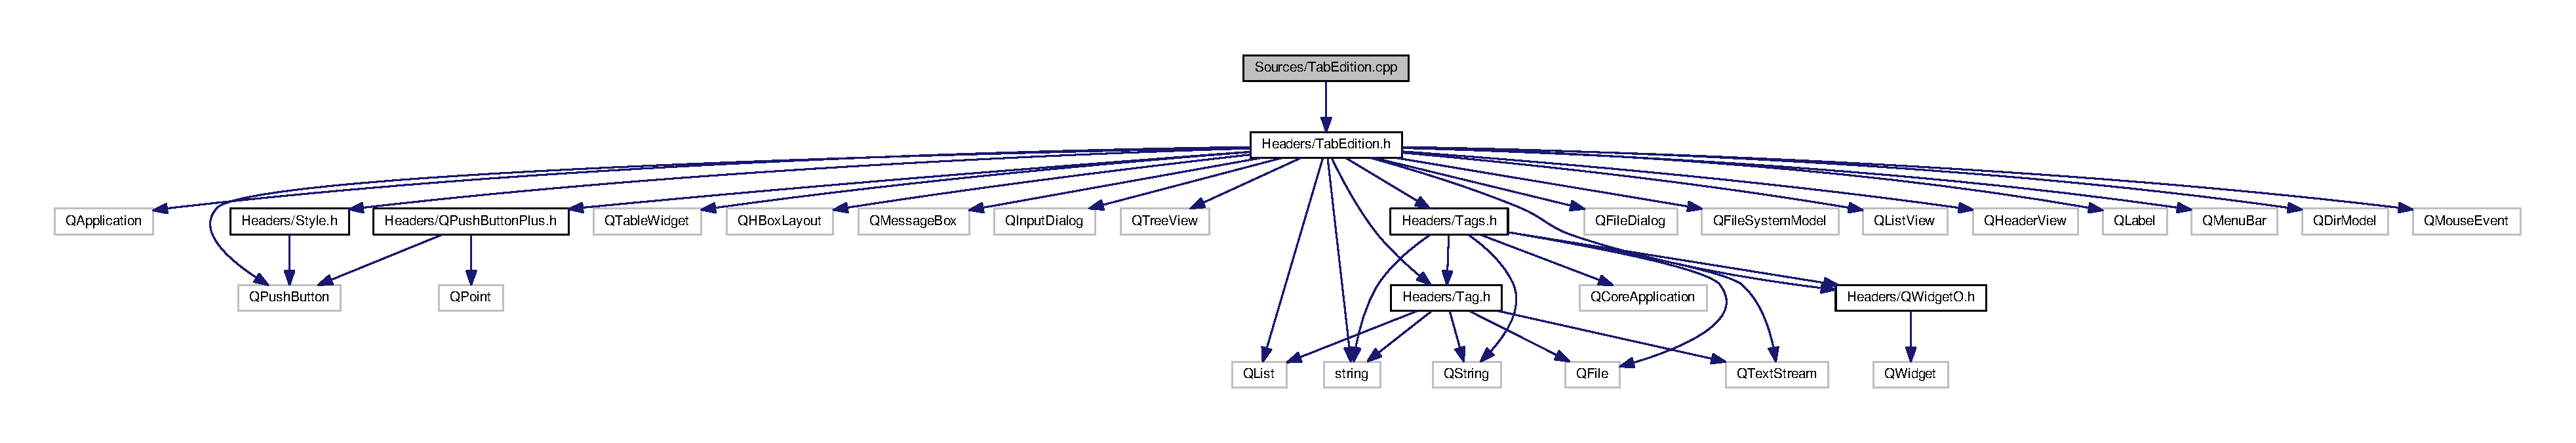
\includegraphics[width=350pt]{_tab_edition_8cpp__incl}
\end{center}
\end{figure}


\subsection{Description détaillée}
implémentation des méthodes de la classe \hyperlink{class_tab_edition}{Tab\+Edition} 

\begin{DoxyAuthor}{Auteur}
G. Killian, P. Sullivan 
\end{DoxyAuthor}
\begin{DoxySince}{Depuis}
14/03/2017 
\end{DoxySince}

\hypertarget{_tab_recherche_8cpp}{}\section{Référence du fichier Sources/\+Tab\+Recherche.cpp}
\label{_tab_recherche_8cpp}\index{Sources/\+Tab\+Recherche.\+cpp@{Sources/\+Tab\+Recherche.\+cpp}}


implémentation des méthodes de la classe \hyperlink{class_q_push_button_plus}{Q\+Push\+Button\+Plus}  


{\ttfamily \#include \char`\"{}Headers/\+Tab\+Recherche.\+h\char`\"{}}\\*
Graphe des dépendances par inclusion de Tab\+Recherche.\+cpp\+:\nopagebreak
\begin{figure}[H]
\begin{center}
\leavevmode
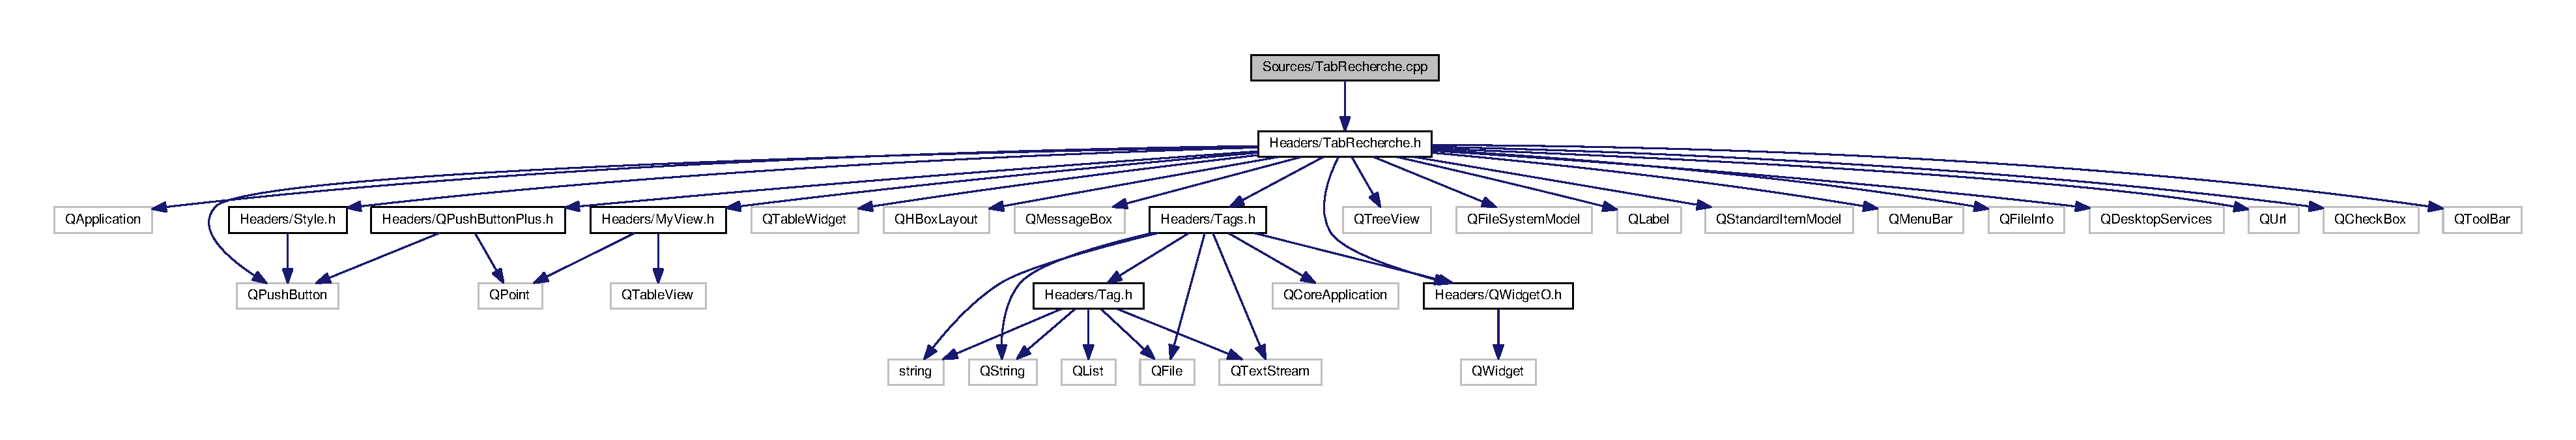
\includegraphics[width=350pt]{_tab_recherche_8cpp__incl}
\end{center}
\end{figure}


\subsection{Description détaillée}
implémentation des méthodes de la classe \hyperlink{class_q_push_button_plus}{Q\+Push\+Button\+Plus} 

\begin{DoxyAuthor}{Auteur}
G. Killian, P. Sullivan 
\end{DoxyAuthor}
\begin{DoxySince}{Depuis}
14/03/2017 
\end{DoxySince}

\hypertarget{_tags_8cpp}{}\section{Référence du fichier Sources/\+Tags.cpp}
\label{_tags_8cpp}\index{Sources/\+Tags.\+cpp@{Sources/\+Tags.\+cpp}}


implémentation des méthodes de la classe Tabs  


{\ttfamily \#include \char`\"{}Headers/\+Tags.\+h\char`\"{}}\\*
Graphe des dépendances par inclusion de Tags.\+cpp\+:\nopagebreak
\begin{figure}[H]
\begin{center}
\leavevmode
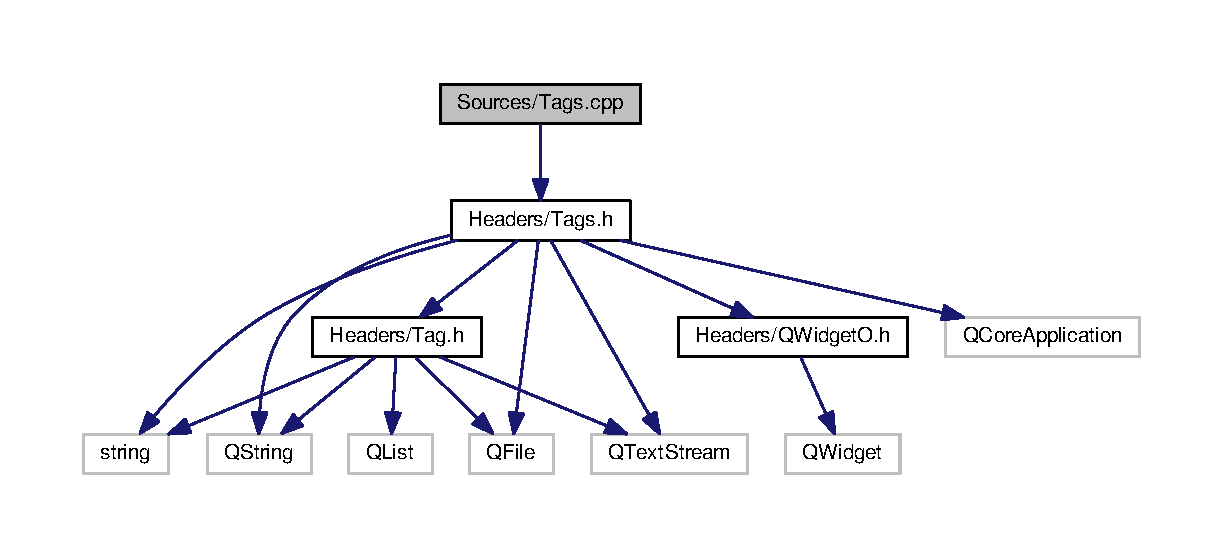
\includegraphics[width=350pt]{_tags_8cpp__incl}
\end{center}
\end{figure}


\subsection{Description détaillée}
implémentation des méthodes de la classe Tabs 

\begin{DoxyAuthor}{Auteur}
G. Killian, P. Sullivan 
\end{DoxyAuthor}
\begin{DoxySince}{Depuis}
14/03/2017 
\end{DoxySince}

%--- End generated contents ---

% Index
\backmatter
\newpage
\phantomsection
\clearemptydoublepage
\addcontentsline{toc}{chapter}{Index}
\printindex

\end{document}
